
\chapter[Estado del Arte]{Simulación de Materiales en Computación Gráfica: Estado del Arte}
\section{Introducción} %(hablar de los diferentes materiales, cómo los modelos "fáciles" no sirven)

En este capítulo se presenta el estado del arte en modelado y renderización de materiales en computación gráfica, junto a un resumen de los aspectos más preponderantes que se deben considerar a la hora de diseñar modelos de los mismos: la geometría a distintas escalas y la  interacción de éstas con fenómenos lumínicos.

Se comienza presentando el marco conceptual sobre la apariencia de los materiales en computación gráfica.
Luego se presentan modelos de la geometría de distintos materiales, desde un punto de vista puramente fenomenológico.
Seguidamente incorporaremos comportamiento físico relacionado al comportamiento o formación del material en consideración.
Luego presentaremos las ecuaciones fundamentales del renderizado, las cuales modelan la interacción entre la energía radiante de la luz en una escena y los materiales que se buscan renderizar.
Finalmente, explicaremos brevemente casos particulares de la ecuación del renderizado que han sido utilizados como estándar en la síntesis de la apariencia de los materiales, y presentaremos ejemplos de algunos materiales que, debido a diversos factores, deben considerar otros métodos menos tradicionales para lograr un renderizado adecuado.
Se muestran ejemplos de materiales cuya síntesis se ajustan a los métodos 
siendo descriptos.

\section{Apariencia de los Materiales}
Entendemos por {\em apariencia} de un material a la percepción del mismo por parte de una persona.
En computación gráfica, se pretende simular de la manera más realista posible las diferentes apariencias.
La apariencia de un material se codifica en aplicaciones gráficas por medio de datos, estructuras de datos y algoritmos, los cuales permiten representar las mismas.

La idea subyacente en la producción de modelos sintéticos de materiales está representada por la síntesis de imágenes capaces de generar el mismo efecto producido por la observación directa de los materiales.
Entre los fenómenos intervinientes en los procesos descriptos, se encuentran la física de la luz y la percepción humana, la cual depende de varios factores.
La consideración de la percepción en el diseño de la apariencia de los materiales ayuda a perfeccionar los modelos existentes, siendo útil para focalizar los esfuerzos de diseño en los elementos más preponderantes intervinientes en dicho fenómeno.
 


\subsection{Escenas y materiales}
Una escena es {\em renderizada} en una computadora por medio de una imagen.
Las dificultades involucradas en el renderizado pueden entenderse mejor si se consideran los cómputos que deben llevarse a cabo.
Típicamente la apariencia de cada punto en una escena depende de objetos que se encuentran a todas las distancias, desde grandes distancias (por ejemplo el Sol), hasta objetos dentro de una misma habitación.

Una imagen sintética se construye discretizando en cada píxel la radiancia proveniente en dirección al observador.
La luz que viaja desde un objeto hacia el observador depende fuertemente del objeto sobre el que la observación sea realizada.
Las propiedades claves del objeto, que determinan la energía lumínica que llega a la cámara, son la {\em forma} y el {\em material} del objeto.

La forma del objeto refiere a su geometría macroscópica.
Las pequeñas imperfecciones de esta geometría también deben ser modeladas para alcanzar una imagen sintética realista.

El material que define el objeto debe modelarse a diferentes escalas y debe poseer determinadas propiedades.
Entre los atributos que componen un material encontramos su color, su función de distribución de energía lumínica, sus texturas, etc.

Existe un compromiso en la elección del modelado de la microgeometría de un material.
Es decir, la elección responde a si se utiliza el modelado geométrico directo (es decir como parte de su forma global), o el modelado de las mismas se incorpora a su material.
La respuesta final depende del material, ya que para algunos de ellos resulta más adecuado modelar la geometría, mientras que la complejidad en la superficie de determinados materiales hacen prohibitivo este enfoque.
Si las micro-geometrías se diseñan en el material, la teoría óptico-geométrica puede ser reemplazada por modelos más precisos (cuánticas, de ondas), posiblemente con consideraciones estadísticas, buscando obtener una aproximación más adecuada a su comportamiento.
Dicho comportamiento se encapsulará en una función de distribución de radiancia sobre la superficie del objeto.



\subsection{Luz}%, complejidad de una escena y percepción.}
La comprensión del fenómeno denominado {\em luz} ha evolucionado a lo largo de la historia humana.
Existen diversos modelos, los cuales atienden a distintas manifestaciones de la misma.
A pesar de los esfuerzos dedicados a lo largo de siglos, la naturaleza de la misma aún no es comprendida en su totalidad, acuñándose el término {\em dualidad onda-partícula} para describirla, debido a que en determinados experimentos la misma parece mostrar propiedades características y concluyentes que permiten catalogarla como una partícula (fotón), mientras que en otros se comporta como una onda.

La luz visible es el sub-fenómeno de la luz que interviene mayormente en la apariencia de los materiales, dado que, debido a limitaciones del sistema de visión, los humanos sólo percibimos los efectos del sub-fenómeno mencionado.
Formalmente la luz visible se define como el rango del espectro de radiación electromagnética entre los  $380${\em nm} y los $780${\em nm}.

Debido al comportamiento dispar del fenómeno lumínico a distintas escalas, debe limitarse el modelado de la misma en una escena, al menos como primera aproximación, a la escala humana.
En dicha escala, la teoría geométrico-óptica de la luz es la que mejor explica el comportamiento de la misma.
En esta representación la luz viaja en línea recta, líneas que son llamadas rayos, los cuales interaccionan con los objetos de una escena, antes de arribar al observador.
La interacción de los rayos con otros objetos produce además rayos secundarios (de refracción, entre otros).

\subsection{Percepción y Color}
El {\em color} de un objeto representa una distribución de radiación electromagnética en el rango de la luz visible.
Una representación realista del color de un material debe modelar al mismo en todas las frecuencias electromagnéticas de la luz visible.
Sin embargo, estudios sobre la formación del color en la visión humana demuestran que el mismo detecta colores gracias a tres canales principales, y la combinación de éstos.
En computación gráfica este conocimiento es tomado en consideración, y aproximado por medio de modelos de espacios cromáticos de tres dimensiones, como por ejemplo \acrshort{RGB}, \acrshort{HSV}, CIELab, etc.

Es de mayor importancia también considerar cuáles aspectos afectan la percepción de un determinado material.
Se habla de materiales {\em rugosos}, {\em brillantes}, {\em opacos}, {\em transparentes}, {\em texturados}, etc.
Estas apariencias responden a estructuras subyacentes en los mismos.
Utilizando estas categorías, previamente definidas por las personas, es posible obtener métodos adecuados para familias de materiales específicos.

\section{Modelos de Geometría de Materiales}
En esta sección presentaremos distintos modelos geométricos de materiales que han hecho su aparición a lo largo de los años en computación gráfica.
Los mismos son el resultado de un balance entre el realismo buscado, los tiempos de cómputo y los recursos de memoria utilizados, y las dificultades en la recolección de datos reales (por ejemplo, detalles microscópicos del material).
La experiencia sugiere que un correcto modelo de la geometría involucrada, posiblemente a distintas escalas, es indispensable para lograr imágenes realistas de los materiales a ser renderizados.

Se comienza describiendo modelos fenomenológicos, para luego incorporar comportamiento físico a los mismos.

\subsection{Modelos Procedimentales}
Un modelo procedimental resulta útil en determinadas situaciones donde la supervisión humana repetitiva no es adecuada o necesaria.
Por ejemplo, si necesita diseñarse un bosque, puede resultar muy costoso económicamente que un artista diseñe cada árbol del mismo, o bien el tiempo necesario puede ser prohibitivo.

Los modelos procedimentales de construcción de geometrías delegan la responsabilidad a un procedimiento o algoritmo automático.
Estos procedimientos cuentan con parámetros que permiten guiar el proceso, pero es finalmente el algoritmo el que obtiene la representación final.
Las principales ventajas de este modelado incluyen el ahorro en memoria (ya que no deben precomputarse las geometrías, sino que se calculan al momento de ser utilizadas), y como fue explicado, la automatización del proceso.

Existen numerosos ejemplos donde se aplica una técnica de modelado procedimental.
En las siguientes sub-secciones presentaremos los ejemplos más ilustrativos, los cuales constituyen estándares actuales en el modelado de dichos materiales.
Si bien los resultados obtenidos presentan gran realismo, los modelos utilizados no tienen una base física, por lo cual luego se muestra un ejemplo de la utilización de modelos físicos para el diseño de materiales, añadiendo en ese caso la posibilidad de predecir la apariencia y comportamiento del mismo.


\subsection{Plantas}
El modelado procedimental de plantas está basado en una interpretación de una tortuga que se mueve por un plano o el espacio tridimensional, dibujando líneas, construyendo de esta manera la geometría de sus ramificaciones \cite{Prusinkiewicz1986}.

Las gramáticas formales \cite{Chomsky1956} intentaron describir el lenguaje natural de forma matemática, por medio de un proceso repetitivo donde sub-cadenas de caracteres son reemplazadas por otras.
Siguiendo esta idea, los sistemas-L \cite{Lindenmayer1968} realizan una descripción algorítmica de la geometría de las plantas.
El concepto central que permite entender el modelado procedimental utilizando sistemas-L es el de {\em reescritura}.
La reescritura consiste en una aplicación sucesiva de reglas que reemplazan determinadas partes en una descripción matemática por otras.
En un sistema-L, una cadena de caracteres representa la estructura de la planta.

Por medio de un proceso repetitivo de reescritura, una cadena de caracteres inicial se transforma, a través de ciertas reglas que deben proveerse, en una cadena final, la cual será interpretada por el algoritmo de la tortuga previamente descripto, produciendo una geometría que asemeja a una planta.

\subsubsection{Definición de sistema-L}
Sea $V$ un alfabeto (conjunto de caracteres), $V^{*}$ el conjunto de todas las palabras que se pueden formar con $V$ y $V^{+}$ el conjunto de todas las palabras que se pueden formar con $V$ y no son vacías.

Una sistema-L de cadenas es una tripleta $G = (V,\omega,P)$, donde $V$ es el alfabeto, $\omega \in V^{+}$ es una cadena no vacía llamada {\em axioma} y $P \subset V \times V^{*}$ es un conjunto finito de reglas de producción.
Una producción $(a,\chi)$ se denota $a \rightarrow \chi$.
$a$ es llamado el {\em predecesor} y $\chi$ el {\em sucesor} de la producción.
Si no se especifica ninguna producción para $a$, se asume $a \rightarrow a \in P$.

Sea $\mu = a_{1}, \dots, a_{m}$ una palabra en $V$.
Se dice que la palabra $\eta = \mu_{1}, \dots, \mu_{m}$ es {\em derivada directamente} de $\mu$, y se nota $\mu \Rightarrow \eta$,  si y sólo si $a_{i} \rightarrow \mu_{i}, \forall i = 1, \dots, m$.

Una palabra $\eta$ es generada por $G$ si existe una secuencia de cadenas que conducen a $\eta$ desde el axioma, es decir, $\beta_{1},\dots,\beta_{n}$, de tal forma que $\beta_{1} = \omega$, $\beta_{n} = \eta$ y $\beta_{1} \Rightarrow \dots  \Rightarrow \beta_{n}$.

Exponemos un ejemplo de generación a continuación.
Si el axioma es $\omega = a$, y las reglas de producción son:
\begin{align*}
p1 &: a \rightarrow b,\\
p2 &: b \rightarrow ab,
\end{align*}

entonces una cadena de derivaciones podría resultar $a \Rightarrow b \Rightarrow ab \Rightarrow bb \Rightarrow abab \Rightarrow \dots$, donde las reglas aplicadas en cada paso serían $p1, p2, p1, p2$ (dos veces).

Estos sistemas fueron diseñados buscando representar las divisiones celulares existentes en ciertas amebas.
Sin embargo, luego se mostrará que los mismos pueden ser utilizados como modelos para capturar la geometría de diversos objetos.

\subsubsection{Interpretación de Tortuga}
Una vez formada una palabra por medio de un sistema-L, la misma debe convertirse en una representación gráfica para poder simular la geometría de la planta.
Para esto se cuenta con la {\em interpretación de tortuga} de la cadena de caracteres.

El estado de la tortuga se define por una tripleta $(x,y,\alpha)$, donde $x,y$ representan la posición de la tortuga en el plano y $\alpha$ es el ángulo hacia donde {\em apunta} la tortuga.
Dado un tamaño de paso $d$ y un incremento angular de $\delta$, la tortuga se ``programa'' para interpretar cadenas de caracteres de la siguiente manera,

\begin{itemize}
\item F, moverse hacia adelante un paso $d$, dibujando,
\item f, moverse hacia adelante un paso $d$, sin dibujar,
\item +, rotar un ángulo $\delta$,
\item -, rotar un ángulo $-\delta$.
\end{itemize}

Al interpretarse el comando $F$, el nuevo estado de la tortuga será $(x',y',\alpha)$, donde $x' = x + d * cos(\alpha)$ y $y' = y + d * sin(\alpha)$. Se dibuja además una línea entre $(x,y)$ y $(x',y')$.
Al interpretarse el comando $f$ ocurre lo mismo, sólo que la línea no se dibuja.
Cuando se lee el comando $+$ (girar a la izquierda). el nuevo estado pasa a ser $(x,y,\alpha-\delta)$ y cuando se interpreta $-$ (girar a la derecha), el nuevo estado resulta $(x,y,\alpha+\delta)$.

De esta forma, dada una cadena $\eta$, la interpretación de tortuga de la misma es la imagen que se genera al responder la tortuga a los comandos inducidos por $\eta$.
La Fig.~\ref{fg:tortuga} muestra un ejemplo de la figura resultante de la cadena FFF-FF-F-F+F+FF-F-FFF, donde la tortuga comienza {\em mirando} hacia arriba, es decir $\delta = 90^{\circ}$.

\begin{figure}
\center
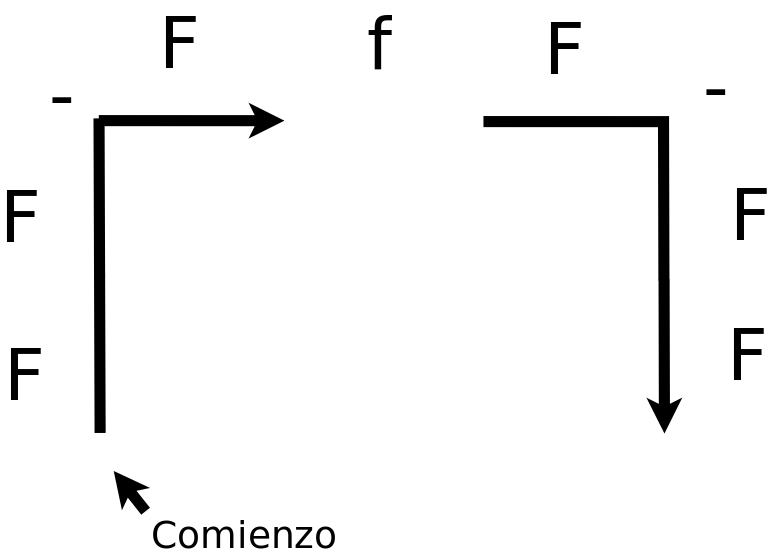
\includegraphics[width=8cm]{figures/tortuga}
\caption{Resultado de la interpretación de tortuga de una cadena de caracteres.}
\label{fg:tortuga}
\end{figure}

La Fig.~\ref{fg:sistemasL} muestra otros ejemplos de sistemas-L, en los cuales se puede observar que con pocas reglas es posible obtener estructuras complejas y de gran belleza.

Usualmente, y debido a la utlización de recursión y repetición, estos sistemas dan lugar a figuras fractales (similares a distintas escalas), por lo cual se las utiliza para dibujar este tipo de estructuras.

\begin{figure}
\center
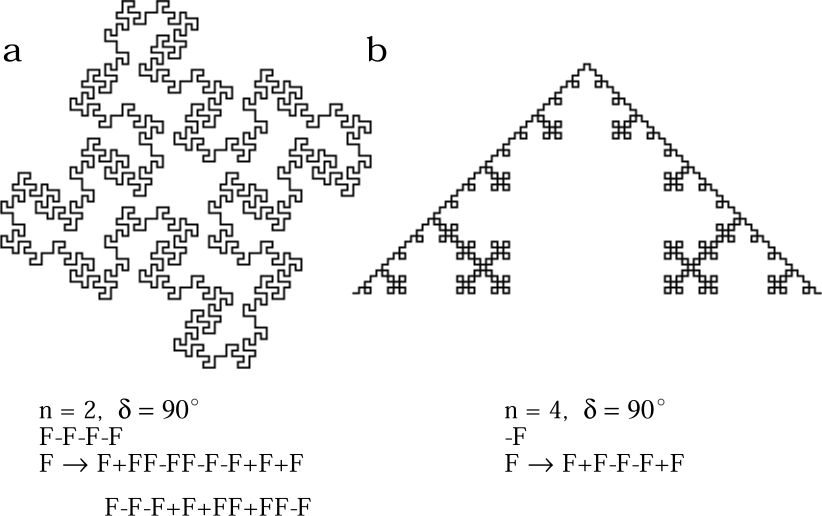
\includegraphics[width=13cm]{figures/sistemasL}
\caption[Sistemas-L generados utilizando distintos parámetros]{Sistemas-L generados utilizando distintos parámetros y una única regla de producción. $n$ es la cantidad de derivaciones utilizadas para producir la cadena que da origen a la figura. En (a), el axioma es F-F-F-F, mientras que en (b) es -F.}
\label{fg:sistemasL}
\end{figure}

Para lograr una imagen que semeje la estructura de árboles y plantas, es necesario introducir dos nuevos caracteres, los cuales son utilizados para generar estructuras ramificadas.
Utilizando una {\em pila} de estados, es posible alcanzar este comportamiento.

El caracter $[$ se utiliza para copiar el estado actual en la pila (operación {\em push}).
De manera análoga, el caracter $[$ implica un reemplazo del estado actual por el de la cabeza de la pila ({\em pop}).
El estado actual de la tortuga está representado por la tripleta antes mencionada.
Por lo tanto, al realizar la operación $]$, en general la posición y orientación de la tortuga cambiarán.
La utilización de un par $[\dots]$ produce que la tortuga dibuje una rama y vuelva al punto inicial, permitiendo continuar con la computación de otras partes de la estructura.

La Fig.~\ref{fg:sistemasLcorchete} muestra ejemplos de gramáticas que producen geometrías visualmente muy similares a plantas.
Por medio de una única regla de producción es posible obtener distintas plantas, y por medio del número de iteraciones se controla cuánto detalle se producirá en la planta (a mayor número de iteraciones, mayor detalle).

\begin{figure}
\center
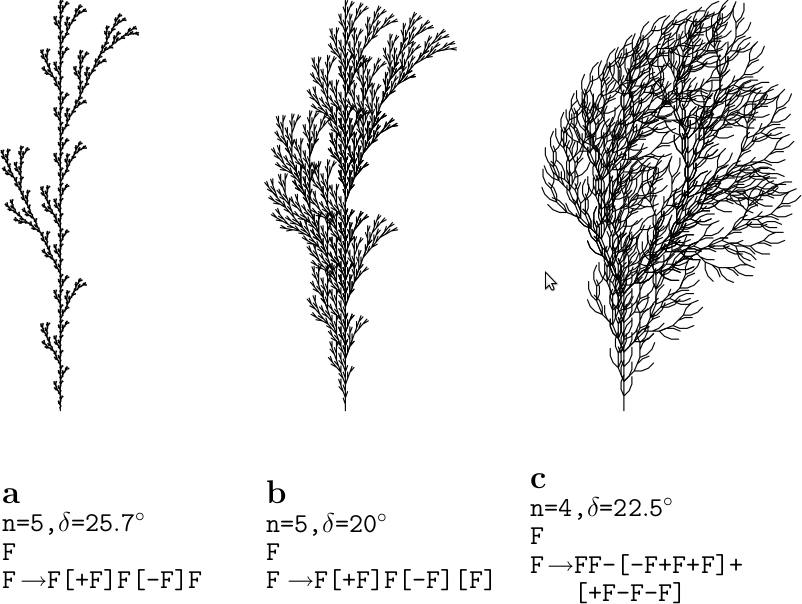
\includegraphics[width=11cm]{figures/sistemalcorchete}
\caption[Sistemas-L con pila de estados, utilizando distintos parámetros]{Sistemas-L con pila de estados, utilizando distintos parámetros. Las imágenes muestran estructuras muy parecidas a plantas. $n$ es la cantidad de derivaciones utilizadas para producir la cadena que da origen a la figura.}
\label{fg:sistemasLcorchete}
\end{figure}


Debido a la facilidad de diseño de nuevas estrategias, y a la naturaleza fenomenológica del método, se han desarrollado numerosas variantes a estos sistemas, los cuales intentan capturar características como mayor aleatoriedad, la aparición de hojas, flores, etc.
Por ejemplo, podría diseñarse una flor como un conjunto de líneas con forma de estrella, y encapsularse a las mismas en una producción de la gramática.
Cuando se desea que se vea una flor, se aplica esta regla.


Entre las especializaciones encontramos sistemas-L estocásticos, los cuales eligen reglas de reescritura de acuerdo a una probabilidad asignada a cada regla, sistemas-L paramétricos, los cuales varían el ángulo y el paso a dibujar dependiendo de la posición de la cadena donde se encuentran, entre otros.
Además, el método es fácilmente generalizable en tres dimensiones, ver Fig.~\ref{fg:sistemasL3D}.
La generalización se realiza por medio de la utilización de matrices de rotación, con un número agregado de operaciones de giro, ver \cite{Prusinkiewicz1990} para obtener mayores detalles.

\begin{figure}
\center
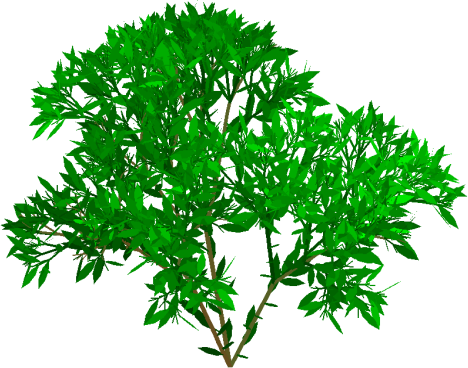
\includegraphics[width=11cm]{figures/3dlsystem}
\caption[Sistema-L en tres dimensiones.]{Planta generada por un sistema-L en tres dimensiones.}
\label{fg:sistemasL3D}
\end{figure}

\subsection{Edificios y Ciudades}
Como fue comentado, una de las ventajas del modelado procedimental es la capacidad de realizar el proceso automáticamente, ahorrando costos y tiempos de diseño.
Un modelado procedimental de edificios puede observarse en \cite{Wonka2003}.
Dicho trabajo presenta un proceso automático que genera de manera casi instantánea edificios arquitectónicamente coherentes, es decir, con ciertas características estructurales que deben ser respetadas.

La diferencia principal a la hora de utilizar sistemas-L para modelar edificios, es que los mismos no pueden ser modelados como una estructura que crece, sino que deben tratarse como conjuntos de objetos con una disposición específica.

Para lograr esto, en \cite{Wonka2003} se proponen varias definiciones, entre las que se encuentran gramáticas de división y gramáticas de control.



Una gramática puede ser definida de manera general como un álgebra de objetos $(U,+,-,F,\leq)$, cerrada bajo las operaciones $+$ y $-$, junto a un conjunto de operaciones $F$, de tal forma que si $u$ y $v$ son miembros de $U$, entonces $u+f(v)$ y $u-f(v)$ lo son, donde $f \in F$.

Una gramática $G=(N,T,R,I)$ es una tupla que consta de cuatro elementos, donde $N \subset U$ representa los nodos no terminales (es decir que se pueden seguir realizando divisiones), $T \subset U$ los terminales (no se pueden dividir), $I \subset N$ un conjunto de objetos iniciales y $R \subseteq U \times U$ un conjunto de producciones.

%Para comprender mejor estos conceptos, definimos una gramática de conjuntos.
%Este tipo de gramáticas 


Una {\em forma} es un conjunto de líneas rectas en el espacio.
Las gramáticas de división seleccionan reglas para subdividir formas en formas más básicas (cubos, cilindros, etc.).

La Fig.~\ref{fg:splitgrammar} muestra un ejemplo del proceso involucrado en una gramática {\em de división}, en la cual una {\em forma} es dividida en otras, utilizando reglas definidas por dicha gramática, en este caso formando una secuencia de ventanas.
Como puede observarse, una gramática de este tipo divide de forma completa el espacio de cada forma, en sub-formas de la misma.

Cuando el proceso llega a su fin, es decir, no existen nodos no terminales ($N$) en el desarrollo, entonces lo que se tiene es un {\em diseño} final.
La principal diferencia con los sistemas-L se basa en que en aquellos, las reescrituras no necesariamente ocupaban el mismo volumen, como sí debe ocurrir en estas gramáticas.

\begin{figure}
\center
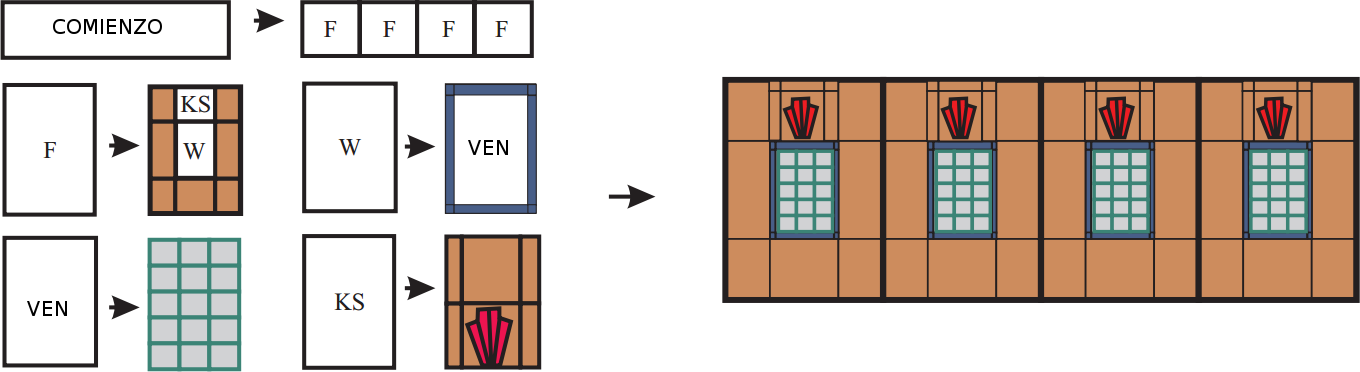
\includegraphics[width=13cm]{figures/splitgrammar}
\caption[Gramática para formar una secuencia de ventanas]{Gramática de división mostrando los pasos seguidos para formar una secuencia de ventanas.}
\label{fg:splitgrammar}
\end{figure}

Las texturas, colores y otras decisiones pueden controlarse por medio de {\em atributos}.
Estos resultan útiles para mantener la coherencia en un mismo piso, por ejemplo, o asegurar que todas las columnas del edificio seguirán un mismo diseño arquitectónico.
Cada símbolo de la gramática es aumentado entonces con uno o más atributos, los cuales especifican estas características para cada parte de la geometría.


Las {\em gramáticas de control} permiten obtener control sobre la distribución de los atributos, y tomar decisiones de diferenciación sobre las divisiones, generando aleatoriedad en los edificios resultantes.
Por ejemplo, se puede requerir que la apariencia del primer piso de un edificio sea diferente al resto (por ejemplo el color, o que sean visibles negocios en la fachada).

Estas gramáticas se invocan a partir de una división específica en una gramática de división.
Cuando se invocan, las mismas generan una secuencia nodos terminales con atributos en la forma $(c,a,v)$, donde $c$ es la posición en la división (fila, columna, capa, en $3D$), $a$ es el atributo y $v$ el valor que tomará.
Estos nodos terminales se utilizan para rellenar los valores de los atributos de las nuevas formas en la división.
Entonces, con una gramática de control es posible controlar el proceso de distribución de atributos.
Un ejemplo sería asignar el atributo {\em puerta} con $1$ a alguna región de la planta baja, y $0$ al resto del edificio.
De igual modo, pueden controlarse los colores de cada piso, seteando por ejemplo colores distintos de manera alternada.
La Fig.~\ref{fg:controlgrammar} muestra un ejemplo de una gramática de control.


Las gramáticas de control también cumplen el propósito de lograr una distribución correcta de las formas.
Por medio de ellas, también es posible {\em excluir} elementos de ciertas posiciones indeseadas (por ejemplo una columna en el último piso), utilizando los mismos atributos para elegir determinadas reglas por sobre otras, logrando un balance de formas en los resultados finales.

El último paso en el sistema es el renderizado, donde una gramática con nodos terminales y atributos se interpreta para generar la imagen del edificio.
Esta interpretación depende de los atributos especificados y puede variar de acuerdo a las necesidades de la aplicación.

\begin{figure}
\center
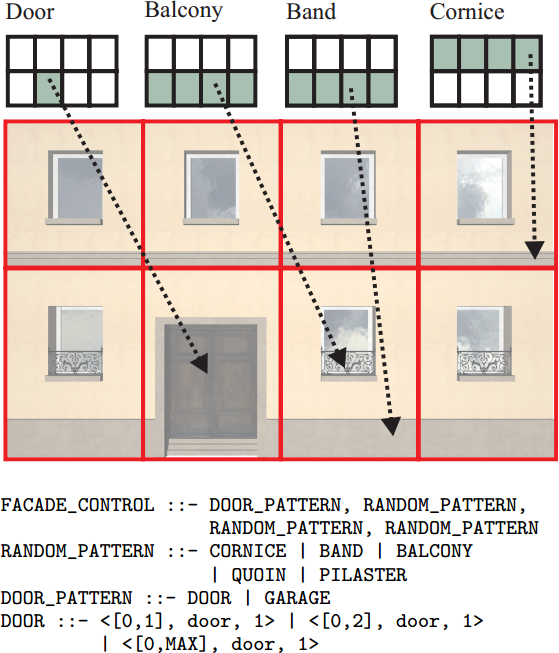
\includegraphics[width=11cm]{figures/controlgrammar}
\caption{Gramática de control.}
\label{fg:controlgrammar}
\end{figure}

La literatura de modelado procedimental de edificios y ciudades ha ido creciendo en los últimos años \cite{Parish2001,Muller2006}.
La Fig.~\ref{fg:edificios} muestra ejemplos de edificios generados procedimentalmente.


\begin{figure}
\center
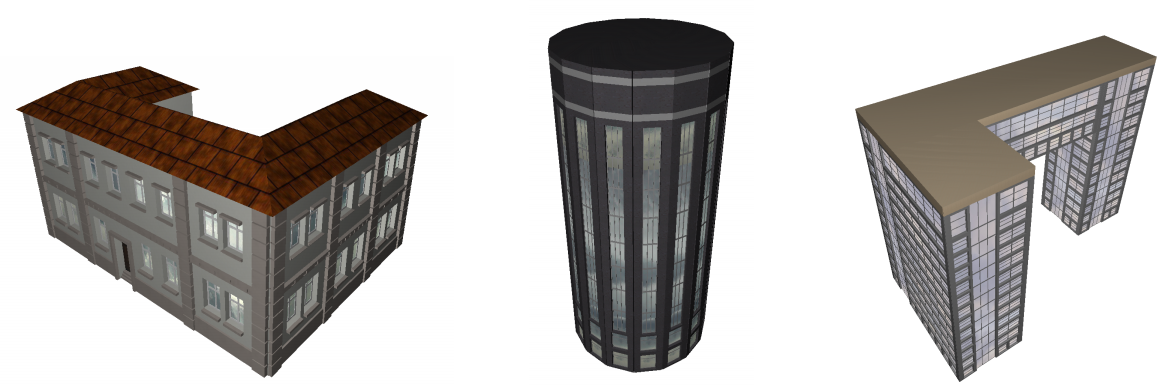
\includegraphics[width=11cm]{figures/edificios}
\caption{Edificios generados procedimentalmente por medio de gramáticas.}
\label{fg:edificios}
\end{figure}

\subsection{Fractales y Montañas}
Una forma de modelar fenómenos de apariencia pseudo-aleatoria (montañas, ríos, nubes) es a través de algoritmos fractales \cite{Mandelbrot1983}.
Al igual que en las secciones anteriores, una única fórmula matemática es lo suficientemente descriptiva como para encapsular todas los detalles, a diferentes escalas, de un fenómeno u objeto dado.
Esto resulta de particular interés en computación, donde los recursos de memoria no son infinitos.

En el siglo $XIX$, el botánico Robert Brown describió el movimiento de partículas de polen en suspensión en agua, a lo cual se le otorgó el nombre de movimiento browniano.
Los movimientos de la partícula se dan sobre direcciones aleatorias por un período de tiempo también aleatorio.
Con el paso de los años se descubrió que la aparente aleatoriedad de los movimientos responde al choque de la partícula de polen con moléculas dispersas en el agua.
Se asume que los movimientos de la partícula de polen son independientes entre sí.

En \cite{Mandelbrot1968}, se plantea una generalización del método llamada movimiento browniano fraccionario (\acrshort{fBm}). 

\begin{align*}
B_{H}(0,w) &= b_{0},\\
B_{H}(u,w)- B_{H}(0,w) &= \frac{1}{\Gamma(H+0.5)} \big\{ \int_{-\infty}^{u} [(u-s)^{H-0.5} - (-s)^{H-0.5} ] dB(s,w) + \\
&  \int_{0}^{u} (u-s)^{H-0.5} dB(s,w) \big \},
\end{align*}


donde $b_{0}$ es un número real, $0 < H < 1$ es el coeficiente de Hurst, $-\infty < u < \infty $ y $w$ es un conjunto de valores aleatorios en un espacio uniforme de muestras.

Cuando $H = 0.5$ se obtiene movimiento Browniano convencional.
En el dominio frecuencial (al cual se puede acceder por medio de una transformada de Fourier), se observa que el fBm no posee una frecuencia dominante, es decir, la función está compuesta por frecuencias a todas las escalas.
Además, la contribución de cada frecuencia es inversamente proporcional a la misma, es decir que el ruido pertenece a la clase de ruidos $\frac{1}{f}$.
El ruido presenta autosimilaridad estadística.
Intuitivamente significa que las características estadísticas del ruido son similares para todas las escalas.

El ruido resulta ser un fractal no determinístico con dimensión $2-H$.
El parámetro $H$ permite simular perfiles con distintas rugosidades.
Cuando $H = 0$, el ruido es indistinguible de un plano.
Cuando $H = 1$, el ruido se transforma en una línea.
Esto resulta útil para modelar perfiles de montañas con distintas rugosidades (más suaves o más pronunciadas), ver Fig.~\ref{fg:hurst}.

\begin{figure}
\center
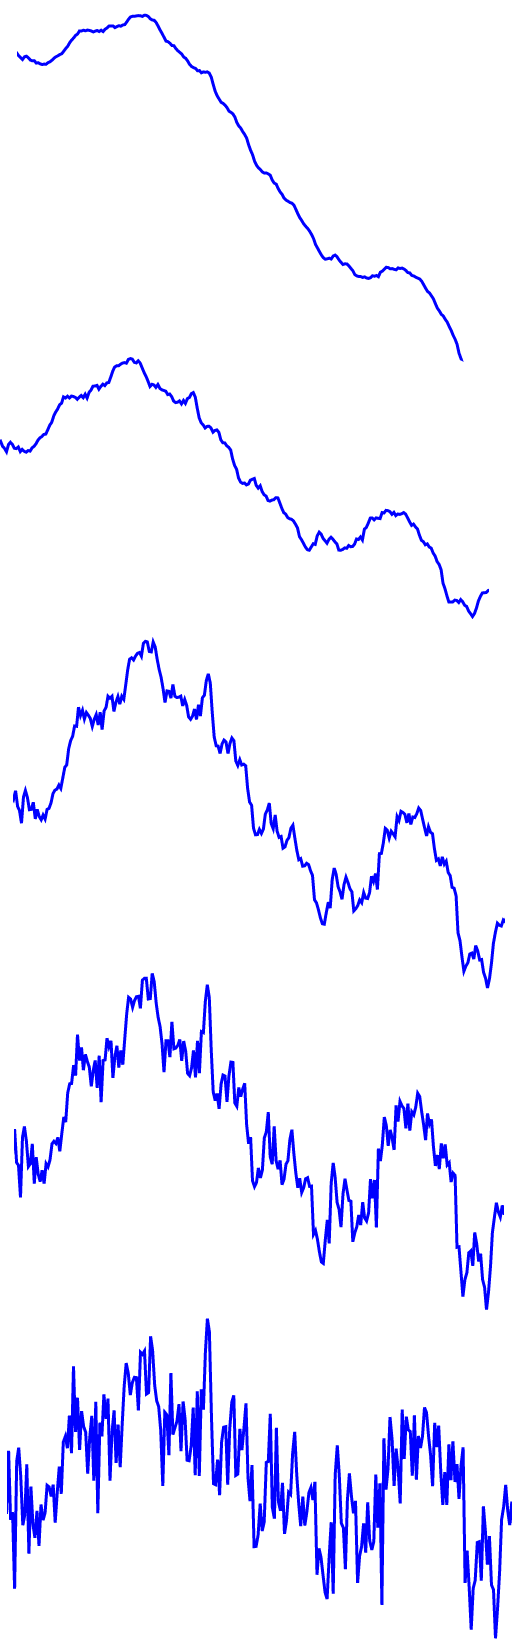
\includegraphics[width=11cm]{figures/hurst}
\caption{Curvas obtenida con distintos coeficientes de Hurst.}
\label{fg:hurst}
\end{figure}

Existen diversos métodos para computar el fBm en computación gráfica.
En \cite{Fournier1982} se presenta un método de subdivisión recursiva, denominado algoritmo de desplazamiento aleatorio del punto medio.

El algoritmo tiene su base en una fórmula de esperanza condicional para $B_{H}(u,w)$ \cite{Mandelbrot1968}.
Partiendo de $B_{H}(0,w) = 0$ y $B_{H}(1,w) = 1$, $0 \le u \le 1$ entonces $E[B_{H}(u,w)|B_{H}(1,w)] = \frac{1}{2} (u^{2H} + 1 - |u-1|^{2H})$.
Si $u=\frac{1}{2}$, entonces la esperanza es igual a $\frac{1}{2}$, independientemente de $H$.
Esto, junto al hecho de que el proceso es autosimilar, permite diseñar un algoritmo que subdivide el segmento en su punto medio, y al valor esperado para el punto medio lo desplaza por un número aleatorio con media $0$ y variancia $1$ multiplicado por la variancia de $B_{H}(u,w)$ en el punto, la cual es igual a $2^{-H}$, en términos matemáticos, $2^{-H} * gauss(0,1) $.
Una vez computado el punto medio, el intervalo se subdivide y se computan de manera recursiva las mitades resultantes, donde la nueva variancia será proporcional al tamaño del nuevo segmento.

En la Fig.~\ref{fg:puntomedio} puede observarse un ejemplo de una curva obtenida utilizando distintas profundidades en el algoritmo recursivo.
Se observa que se puede obtener mayor detalle a mayor número de iteraciones, donde la curva resultante asemeja visualmente al perfil de una montaña.

\begin{figure}
\center
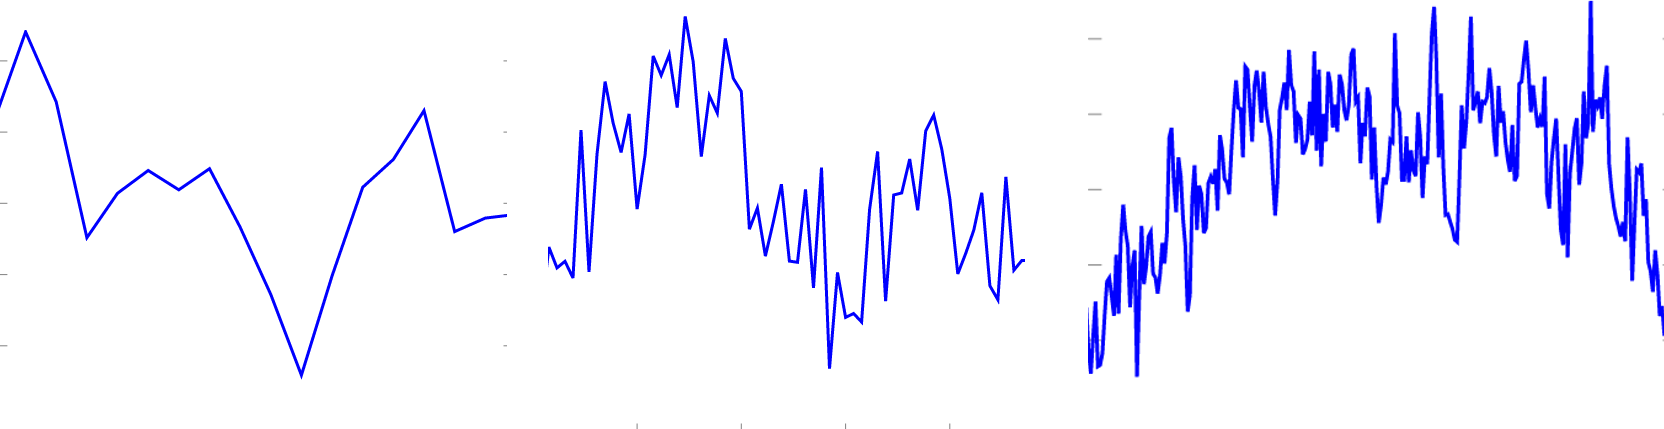
\includegraphics[width=11cm]{figures/puntomedio}
\caption[Curva obtenida utilizando el algoritmo del punto medio]{Curva obtenida con $H=0.8$, para $17$, $65$ y $257$ muestras, utilizando el algoritmo del punto medio.}
\label{fg:puntomedio}
\end{figure}


Una extensión directa de este algoritmo se da en dos dimensiones, donde los valores que se subdividen representan las alturas de un terreno.
Comenzando con $4$ puntos en un plano, formando un cuadrado, donde cada punto almacena la altura del terreno, es posible sudividir el terreno en $4$ cuadrados, a partir de los puntos medios de cada arista del cuadrado original.
Con $H$ es posible controlar la rugosidad del terreno.
La Fig.~\ref{fg:terreno} muestra un ejemplo de la renderización de un terreno generado utilizando este método, donde $H = 0.9$, en la Fig.~\ref{fg:terreno2} $H = 0.3$.
Se puede observar que a medida que $H$ es mayor, el terreno es más suave.

\begin{figure}
\center
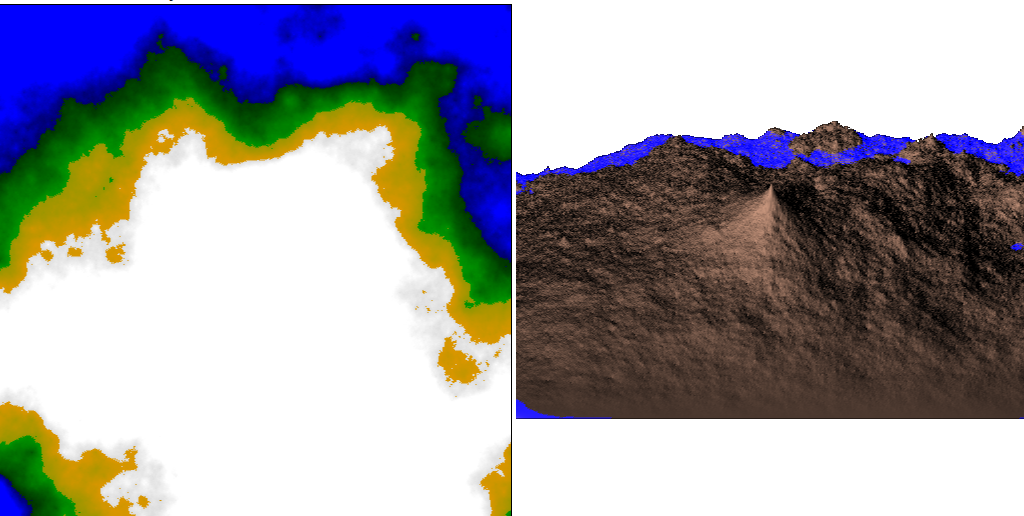
\includegraphics[width=11cm]{figures/terreno}
\caption[Terreno generado utilizando el algoritmo de desplazamiento del punto medio en dos dimensiones, con $H = 0.9$]{Terreno generado utilizando el algoritmo de desplazamiento del punto medio en dos dimensiones, con $H = 0.9$. La imagen de la izquierda muestra colores agregados de acuerdo al número generado, la imagen de la derecha muestra un ejemplo tridimensional de los mismos datos visto en perspectiva.}
\label{fg:terreno}
\end{figure}

\begin{figure}
\center
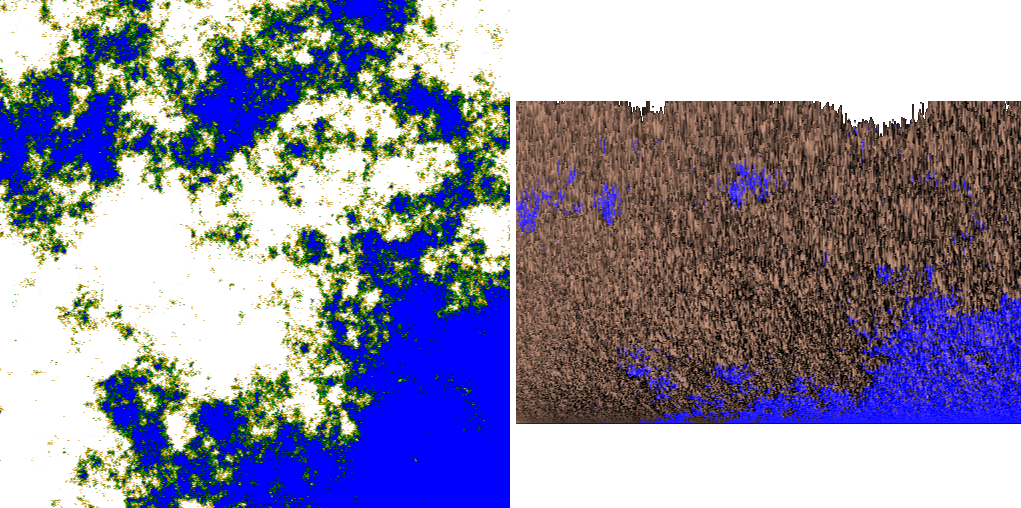
\includegraphics[width=11cm]{figures/terreno2}
\caption[Terreno generado utilizando el algoritmo de desplazamiento del punto medio en dos dimensiones, con $H = 0.3$]{Terreno generado utilizando el algoritmo de desplazamiento del punto medio en dos dimensiones, con $H = 0.3$.}
\label{fg:terreno2}
\end{figure}

%\subsubsection{Planetas}
%\cite{Ebert2002}


\subsection{Modelos Físicos}
Si bien los resultados obtenidos por los modelos presentados hasta ahora son muy satisfactorios, existe aún la necesidad de no depender de parámetros ad-hoc, además de aumentar el realismo de las imágenes resultantes.
Hasta aquí, la utilización de los modelos se basa casi exclusivamente en su {\em parecido visual} a los objetos que se intentan modelar.

Para poder obtener una representación más ajustada a la geometría real de los materiales, es necesario utilizar los procesos físicos de formación o comportamiento de los materiales (movimiento de partículas, deformaciones, cambios químicos, etc.), lo cual permitiría definir parámetros más intuitivos que tienen su correlación en la realidad, logrando además una representación más exacta de la misma.
La desventaja de utilizar modelos físicos o matemáticos, recae sobre los tiempos de cómputo y la dificultad de diseño de éstos.

Sin embargo, desde el surgimiento del área, estos modelos han ido evolucionando gracias al incremento en el poder de cómputo del hardware gráfico disponible. A pesar de esto, aún nos encontramos en los comienzos de la utilización masiva de los mismos, por lo cual existen sólo unos pocos casos en los que se utilizan modelos de primeros principios.
En esta sección presentamos un ejemplo de esto, lo cual ejemplifica la capacidad de representación que puede alcanzarse al agregar detalles reales en las implementaciones.

\subsection{Fluidos}
Entre los primeros intentos por utilizar procesos físicos para modelar la apariencia de los materiales, encontramos ecuaciones que describen fluidos.
Las ecuaciones de Navier-Stokes describen un fluído cuya temperatura es prácticamente constante, por medio de un campo vectorial de velocidades $\bold{u}$ y un campo de presiones $p$.

Dadas condiciones iniciales para $\bold{u}$ y $p$ cuando $t = 0$, la evolución de las cantidades puede describirse como sigue, independientemente del número de dimensiones,

\begin{align}
\nabla \cdot \bold{u} &= 0, \label{eq:eq1}\\
\frac{\partial \bold{u} }{\partial t} &= - (\bold{u} \cdot \nabla) \bold{u} - \frac{1}{\rho} \nabla p + \nu \nabla^{2} \bold{u} + \bold{f} \label{eq:eq2},
\end{align}

donde $\nu$ es la viscosidad cinemática del fluído, $\rho$ es la densidad y $\bold{f}$ es una fuerza externa.
Las ecuaciones modelan la conservación de masa (\ref{eq:eq1}) y de momento (\ref{eq:eq2}).

Además, deben tenerse en cuenta condiciones de borde.
Las mismas pueden variar en complejidad.
Por ejemplo, una implementación sencilla puede darse utilizando condiciones de borde periódicas, es decir, sin la existencia de {\em paredes} (el fluido se repite indefinidamente, este es el caso utilizado en el trabajo descripto aquí).
Un caso más realista lo constituye una condición diferencial que describe el intercambio de masa con el ambiente.

Es posible combinar ambas ecuaciones para obtener una única ecuación de la velocidad.
Para esto, se utiliza la descomposición de Helmholtz-Hodge \cite{Chorin1990}, la cual establece que un campo vectorial $\bold{w}$ puede descomponerse como sigue, 

\begin{equation}
\label{eq:eq3}
\bold{w} = \bold{u} + \nabla q,
\end{equation}

donde $\bold{u}$ tiene divergencia $0$, es decir $\nabla\cdot\bold{u} = 0$.
Entonces, se puede definir un operador $\bold{P}$, el cual proyecta un campo vectorial $\bold{w}$ en su componente de divergencia $0$, $\bold{u} = \bold{P}\bold{w}$.
Dicho operador se puede definir implícitamente multiplicando $\nabla$ en ambos términos en la ecuación (\ref{eq:eq3}),

\begin{equation}
\label{eq:eq4}
\nabla\cdot\bold{w} = \nabla^{2} q.
\end{equation}

Una solución a esta ecuación está dada por

\begin{equation}
\label{eq:eq5}
\bold{u} = \bold{P}\bold{w} = \bold{w} - \nabla q,
\end{equation}

Aplicando el operador $\bold{P}$ en ambos lados de la ecuación (\ref{eq:eq2}), se obtiene una ecuación única para la velocidad,

\begin{equation}
\frac{\partial \bold{u} }{\partial t} = \bold{P} (- (\bold{u} \cdot \nabla) \bold{u} + \nu \nabla^{2} \bold{u} + \bold{f}) \label{eq:eq6},
\end{equation}

ya que $\bold{P}\bold{u} = \bold{u}$ y $\bold{P}\nabla p = 0$.
Esta ecuación es utilizada en la derivación de un algoritmo práctico que implementa apariencia de fluídos \cite{Stam1999}.
En la ecuación pueden verse un paso difusivo $\nu \nabla^{2} \bold{u}$, un paso de advección $- (\bold{u} \cdot \nabla) \bold{u}$ y una fuerza final aplicada $\bold{f}$.
Estos términos pueden resolverse por medio de la aplicación de métodos numéricos clásicos (por ejemplo diferencias finitas), por lo cual la solución final consiste en aplicar sucesivamente cada paso para obtener soluciones al campo vectorial $u$ en cada instante de tiempo $t$, finalmente proyectando el resultado con $P$.
El paso más complicado es el paso de proyección $P$, el cual se resuelve por medio de sistemas lineales, teniendo en cuenta que es una ecuación de Poisson.

Cuando se conocen las velocidades $\bold{u}$, es posible definir un sistema de partículas sobre el fluido, las cuales poseerán las velocidades dadas por $\bold{u}$ de acuerdo a su posición en el medio.
De esta forma se podrá proceder a su renderizado.

Este método se utiliza para modelar el comportamiento de agua y otros líquidos, además de algunos gases, nubes y humo, ver Figs.~\ref{fg:fluidos1},\ref{fg:fluidos2}.

La utilización de los procesos físicos subyacentes produce mayor realismo en las imágenes resultantes sobre la utilización de métodos heurísticos y fenomenológicos.
Desafortunadamente, muchas veces este enfoque resulta prohibitivo, no solo debido a costos computacionales, sino también por la complejidad presente en el diseño de los métodos, ya que se requiere muchas veces la participación de personas provinientes de áreas científicas afines a la física utilizada.


\begin{figure}
\center
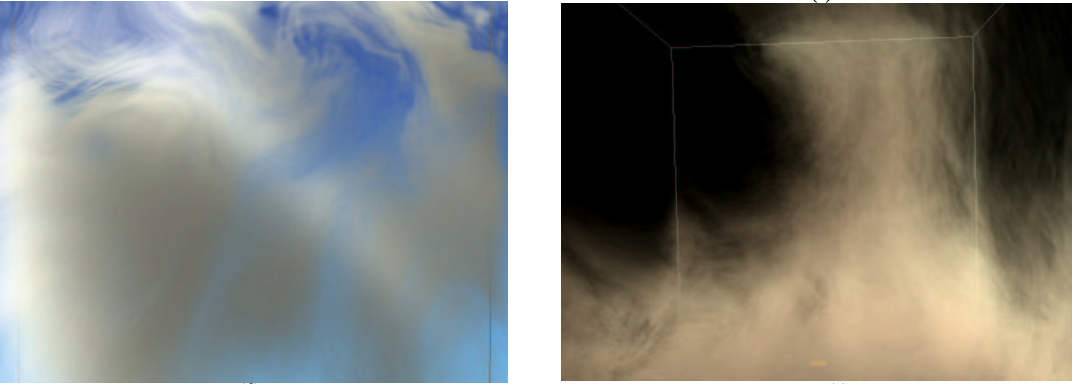
\includegraphics[width=11cm]{figures/fluidos1}
\caption{Nubes y humo generados utilizando métodos basados en las ecuaciones de Navier-Stokes.}
\label{fg:fluidos1}
\end{figure}

\begin{figure}
\center
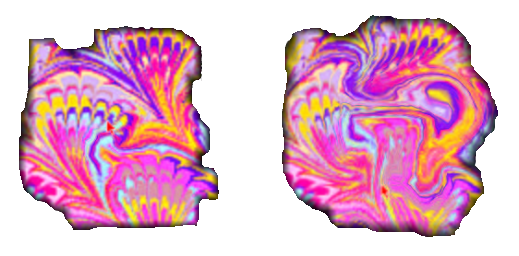
\includegraphics[width=11cm]{figures/fluidos2}
\caption{Fluidos generados utilizando métodos basados en las ecuaciones de Navier-Stokes.}
\label{fg:fluidos2}
\end{figure}

%\subsubsection{Telas}

\section{Representación Visual (Renderizado)}

Además de presentar una geometría compleja, los materiales exhiben fenómenos particulares en su interacción con la luz, entre los cuales se observan translucencia, reflectancia, absorción, etc.
Cada fenómeno puede determinar de forma inequívoca la apariencia de un material determinado.
Debido a esto, en las décadas posteriores al nacimiento de la informática gráfica, se desarrollaron distintas técnicas, inpiradas en determinadas ecuaciones físicas que fueron simplificadas y aproximadas para ser implementadas por medio de una computadora, permitiendo modelar la apariencia de una gran variedad de materiales.

\subsection{Ecuación del Renderizado}

Esta ecuación modela el comportamiento de la luz en una escena y su interacción con distintos tipos de superficies \cite{Kajiya1986}.
La misma se basa en el principio de la conservación de la energía, el cual establece que la energía saliente debe ser igual a la energía entrante, más la energía emitida, menos la energía absorbida.
La ecuación presenta la siguiente definición:

\begin{equation}
L(\bold{x'} \rightarrow \bold{x}) =  g(\bold{x'}  \rightarrow \bold{x})  \left[ \epsilon(\bold{x'}  \rightarrow \bold{x}) + \int_{s}{\rho(\bold{x''}  \rightarrow \bold{x'}  \rightarrow \bold{x})L(\bold{x''}  \rightarrow \bold{x}) d\bold{x''}} \right],
\end{equation}
donde $L(\bold{x'} \rightarrow \bold{x})$ es la intensidad de la luz que viaja del punto tridimensional $\bold{x'}$ al punto $\bold{x}$ (sin oclusiones), $g(\bold{x'} \rightarrow \bold{x})$ es un termino geométrico que modela la oclusión que podría existir entre $\bold{x}$ y $\bold{x'}$, $\epsilon(\bold{x'} \rightarrow \bold{x})$ es la intensidad de la luz emitida desde $\bold{x'}$ a $\bold{x}$, $\rho(\bold{x''}  \rightarrow \bold{x'}  \rightarrow \bold{x})$ es la intensidad de la luz emitida de $\bold{x''}$ a $\bold{x}$ por medio de una superficie en $\bold{x'}$ (esta cantidad será llamada función bidireccional de distribución de reflectancia, \acrshort{BRDF}, en una sección posterior), y $S=\bigcup{s_{i}}$ es la unión de todas las superficies $s_{i}$ de la escena.


Puede observarse que la ecuación presenta una definición recursiva, ya que la energía radiante saliente de un punto $x'$ depende de la energía radiante que llega desde todos los puntos de todas las superficies a ese punto.
De esta forma, $\bold{x}$,$\bold{x'}$ y $\bold{x''}$ varían sobre todas las superficies de la escena.
Además se asume una superficie $S_{0}$, la cual se modela como un semi-hemisferio que engloba a toda la escena.

La ecuación es una aproximación óptico-geométrica a las ecuaciones del electromagnetismo de Maxwell.
$L$ representa la radiación de energía por unidad de tiempo por unidad de superficie de destino por unidad de superficie de origen ($joule/m^{4} s$).
El término geométrico se hace $0$ si los puntos en consideración no son mutuamente visibles.

Por medio del modelado de cada término de forma separada, es posible visualizar fielmente una gran cantidad de superficies.
Trabajos previos a la aparición de la ecuación del renderizado habían alcanzado resultados parciales, pero no habían logrado sintetizar un único método que englobe todos los fenómenos en investigación hasta ese entonces.
Entre los casos particulares de la ecuación del renderizado, los más emblemáticos han sido el trazado de rayos \cite{Whitted1980} y la radiosidad \cite{Goral1984}.
El primero es un método adecuado para renderizar superficies especulares (la luz se refleja en las superficies en direcciones específicas), mientras que la radiosidad es un método diseñado para simular superficies cuyas geometrías microscópicas provocan la distribución de la luz reflejada de manera equitativa, produciendo una apariencia difusa.

Fuera de la ecuación quedan efectos más complejos, como la difracción y la polarización.
Más detalles de la misma pueden ser consultados en \cite{Kajiya1986}.
Un esquema de esta ecuación puede observarse en la Fig. \ref{fg:rendequation}.

\begin{figure}
\center
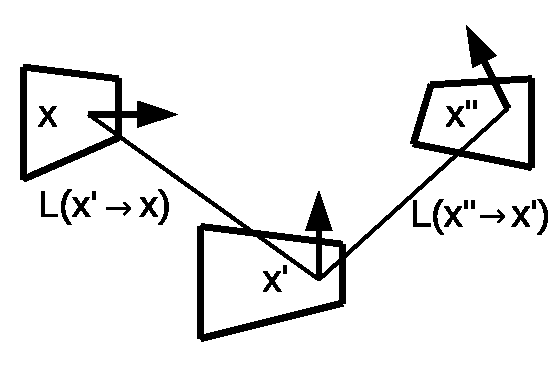
\includegraphics[width=8cm]{figures/rendequation}
\caption[Interpretación visual de la ecuación del renderizado]{Interpretación visual de la ecuación del renderizado (término $L(\bold{x''}  \rightarrow \bold{x}) $). La ecuación modela la distribución de radiancia en una escena, considerando todas las superficies intervinientes. La imagen muestra además los vectores normales a las superficies.}
\label{fg:rendequation}
\end{figure}

La ecuación presentada modela correctamente el comportamiento de la energía radiante en superficies en una escena tridimensional.
Si lo que se pretende modelar son fenómenos volumétricos, como partículas en el ambiente, o materiales transparentes, entre otros ejemplos, entonces deben atenderse ciertas generalizaciones de la ecuación, como se desarrolla en la siguiente sub-sección.

\subsection{Ecuación del Renderizado de Volúmenes}

En esta sección denotaremos como $L(\bold{x} \rightarrow \vec{\omega})$ a la energía radiante o {\em radiancia} que parte desde un punto del espacio $\bold{x}$ en la dirección $\vec{\omega}$.
Siguiendo la notación de la sección anterior, para cada vector en el espacio $\vec{\omega}$, existe un punto tridimensional $\bold{y}$ tal que $L(\bold{x} \rightarrow \vec{\omega}) = L(\bold{x} \rightarrow \bold{y})$.

La luz es modelizada por medio de partículas denominadas {\em fotones}. Cuando un fotón de un rayo de luz atraviesa un medio en una dirección dada, pueden ocurrir una serie de eventos, de los cuales dos corresponden a fenómenos de extinción: la absorción y la redirección del mismo en otra dirección.
Estos fenómenos dependen del coeficiente de absorción del medio $\sigma_{a}$ y el coeficiente de dispersión $\sigma_{s}$.
La suma de ambos se denota como el coeficiente de extinción $\sigma_{t}$.

El coeficiente de absorción en un segmento de recta se denota como $\sigma_{a}(\bold{x} + t\vec{\omega})$.
La fracción de fotones absorbidos en ese segmento de recta es notada como $\sigma_{a}(\bold{x} + t\vec{\omega}) \Delta t$.
Consecuentemente la fracción de fotones que escapa a la absorción en ese segmento de recta resulta $(1-\sigma_{a}(\bold{x} + t\vec{\omega}) \Delta t)$.
Finalmente, podemos escribir la radiancia que {\em escapa} del medio en dirección $\vec{\omega}$ como,

$$L((\bold{x}+t\vec{\omega}) \rightarrow \vec{\omega}) = L(\bold{x} \rightarrow \vec{\omega}) (1-\sigma_{a}(\bold{x} + t\vec{\omega}) \Delta t),$$

o, de otra forma:

$$\frac{L((\bold{x}+t\vec{\omega}) \rightarrow \vec{\omega}) - L(\bold{x} \rightarrow \vec{\omega}) }{ \Delta t } = - \sigma_{a}(\bold{x} + t\vec{\omega}) L(\bold{x} \rightarrow \vec{\omega}).$$

Tomando el límite cuando $\Delta t \rightarrow 0$ se obtiene la derivada, es decir, el cambio diferencial en radiancia dado por la absorción del medio,

$$\lim_{\Delta t \rightarrow 0} \frac{L((\bold{x}+t\vec{\omega}) \rightarrow \vec{\omega}) - L(\bold{x} \rightarrow \vec{\omega}) }{ \Delta t } = (\vec{\omega} \cdot \nabla_{a}) L(\bold{x} \rightarrow \vec{\omega}) = - \sigma_{a}(\bold{x}) L(\bold{x} \rightarrow \vec{\omega}),$$

donde $\nabla_{a}$ denota el gradiente dado por la absorción y $ \vec{\omega} \cdot \nabla_{a}$ expresa la derivada direccional de la absorción del medio en dirección $\vec{\omega}$.

Similarmente se halla el cambio en radiancia debido a la dispersión saliente,

$$ (\vec{\omega} \cdot \nabla_{o}) L(\bold{x} \rightarrow \vec{\omega}) = -\sigma_{s}(\bold{x}) L(\bold{x} \rightarrow \vec{\omega}),$$

de esta forma se pueden aunar ambos términos para expresar el cambio en radiancia debido a la extinción,

$$(\vec{\omega} \cdot \nabla_{t}) L(\bold{x} \rightarrow \vec{\omega}) = -(\sigma_{a}(\bold{x})+\sigma_{s}(\bold{x})) L(\bold{x} \rightarrow \vec{\omega}) = -\sigma_{t}(\bold{x}) L(\bold{x} \rightarrow \vec{\omega}).$$

Gracias a esta expresión se puede calcular una cantidad de interés, llamada {\em Transmitancia}, $T_{r}$, la cual describe la cantidad de fotones que pueden viajar sin obstrucciones entre dos puntos en un medio (en línea recta).
Integrando la ecuación anterior es posible obtener una expresión para la transmitancia,

$$T_{r}(\bold{x'} \leftrightarrow \bold{x}) = e^{-\tau(\bold{x'} \leftrightarrow \bold{x})},$$

donde $\tau$ recibe el nombre de densidad óptica del material y su expresión es,

$$\tau(\bold{x'} \leftrightarrow \bold{x}) = \int_{0}^{d} -\sigma_{t}(\bold{x}+t\vec{\omega})dt,$$

con $t \in [0,d]$.
La ecuación es el resultado de integrar la extinción a lo largo del segmento de recta.


Hasta ahora se describió la pérdida de fotones a medida que un rayo de luz viaja por un medio.
Similarmente existen dos fenómenos que provocan el desvío de fotones hacia la dirección $\vec{\omega}$.
El primero es llamado dispersión entrante, y consiste en el rebote de fotones que provocan que los mismos adopten la dirección del rayo actual.
Su expresión matemática es

$$ (\vec{\omega} \cdot \nabla_{i}) L(\bold{x} \rightarrow \vec{\omega}) = \sigma_{s}(\bold{x}) L_{i}(\bold{x} \rightarrow \vec{\omega}).$$

El último fenómeno ocurre en medios que transforman otras formas de energía como el calor, en luz visible, y se llama emisión, con expresión

$$ (\vec{\omega} \cdot \nabla_{e}) L(\bold{x} \rightarrow \vec{\omega}) = \sigma_{a}(\bold{x}) L_{e}(\bold{x} \rightarrow \vec{\omega}).$$

La ecuación en su forma completa representa el comportamiento de la luz en volúmenes, considerando los cuatro fenómenos \cite{Jarosz2008}:

\begin{equation}
\begin{aligned}
(\vec{\omega} \cdot \nabla) L(\bold{x} \rightarrow \vec{\omega}) = - \sigma_{a}(\bold{x}) L(\bold{x} \rightarrow \vec{\omega}) - \sigma_{s}(\bold{x}) L(\bold{x} \rightarrow \vec{\omega}) + \\
\sigma_{a}(\bold{x}) L_{e}(\bold{x} \rightarrow \vec{\omega}) + \sigma_{s}(\bold{x}) L_{i}(\bold{x} \rightarrow \vec{\omega}).
\end{aligned}
\end{equation}

La misma expresa que el cambio ($\nabla$) de radiancia $L$ de un rayo de luz en un medio, en una dirección dada ($\vec{\omega}$) está dado por cuatro fenómenos: absorción, dispersión saliente, emisión (del medio) y dispersión entrante, ver Fig.~\ref{fg:fenomenosrte}.
Esta ecuación recibe el nombre de ecuación del transporte radiativo (Radiative Transport Equation, \acrshort{RTE}) \cite{Chandrasekhar1960}.

Podemos expresar esta ecuación en forma integral integrando ambos lados de la igualdad, y asumiendo como condición de borde a la ecuación del renderizado de la sección anterior, obteniendo,

\begin{equation}
\begin{aligned}
L(\bold{x} \leftarrow \vec{\omega}) = T_{r}(\bold{x} \leftrightarrow \bold{x_{s}}) L(\bold{x_{s}} \rightarrow -\vec{\omega}) + \\
\int_{0}^{s}{T_{r}(\bold{x} \leftrightarrow \bold{x_{t}}) \sigma_{a}(\bold{x}) L_{e}(x \rightarrow -\vec{\omega}) dt } + \\
\int_{0}^{s}{T_{r}(\bold{x} \leftrightarrow \bold{x_{t}}) \sigma_{a}(\bold{x_{t}}) L_{i}(x_{t} \rightarrow -\vec{\omega})  }
\end{aligned}
\label{eq:rteintegral}
\end{equation}

donde $L(\bold{x} \leftarrow \vec{\omega})$ describe la radiancia que llega a $\bold{x}$ desde $\bold{\omega}$ (este es el caso inverso a $L(\bold{x} \rightarrow {\vec{\omega}})$, el cual resulta útil en el diseño de algoritmos que implementan esta ecuación), $s$ es la profundidad del medio desde $\bold{x}$ en dirección $\vec{\omega}$, $\bold{x_{t}} = \bold{x} + t\vec{\omega}$ con $t \in (0,s)$ y $\bold{x_{s}} = \bold{x}+ s\vec{\omega}$ es un punto en una superficie cercana y visible desde el medio, ver Fig.~\ref{fg:rte}.
El primer término de la ecuación representa radiancia entrando por detrás del medio.
El segundo, la emisión de radiancia en el medio.
El último, la acumulación de radiancia entrante al medio. 
Esta forma integral de la ecuación RTE recibe el nombre {\em Ecuación del Renderizado de Volúmenes}.

Esta ecuación es aún más compleja que la ecuación del renderizado presentada en la sección anterior.
Cada punto del medio depende de {\em todos} los demás puntos del medio, por lo que deben desarrollarse métodos que permitan computar aproximaciones adecuadas de la misma.
Simplificaciones usuales incluyen ignorar el término de emisión, y asumir un medio isotrópico u homogéneo.

Como fue aclarado, diversos algoritmos específicos surgieron con anterioridad a estas ecuaciones generales, y sin saberlo, formaban parte de un mismo marco teórico, las cuales hoy por hoy son algoritmos especializados para ciertos tipos de materiales y situaciones.



\begin{figure}
\center
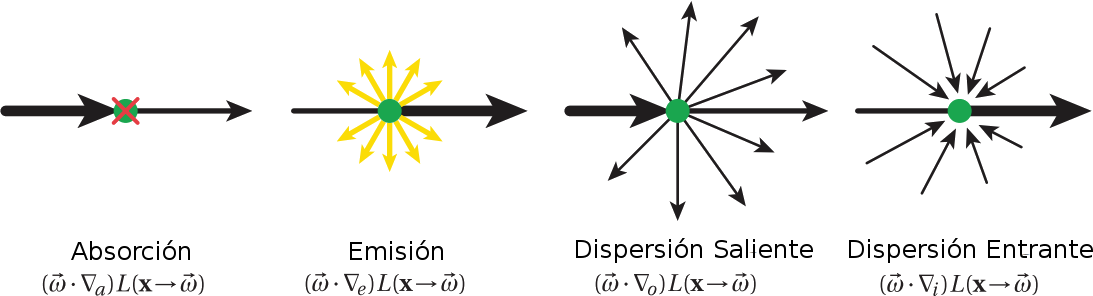
\includegraphics[width=11cm]{figures/fenomenosrte}
\caption{Fenómenos intervinientes en la Ecuación del Transporte Radiativo.}
\label{fg:fenomenosrte}
\end{figure}

\begin{figure}
\center
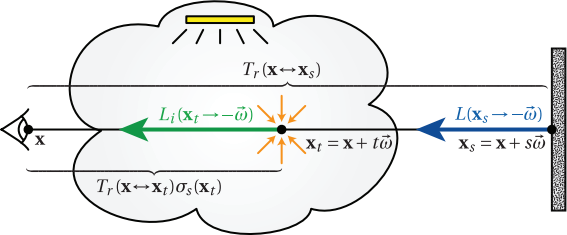
\includegraphics[width=11cm]{figures/rte}
\caption{Interpretación gráfica de la Ecuación del Transporte Radiativo.}
\label{fg:rte}
\end{figure}


%\section{Simplificaciones a las Ecuaciones de Renderizado}
\section{Funciones de Distribución de Reflectancia (BRDFs)}
En la ecuación del renderizado se introdujo un término llamado BRDF, el cual representa una función que modela el comportamiento de la luz en relación con una superficie determinada.
Dada una dirección de entrada y una de salida de un rayo de luz que impacta una superficie, la función devuelve la cantidad de radiancia que emite la superficie en la dirección saliente al recibir energía radiante en su dirección entrante.

\begin{figure}
\center
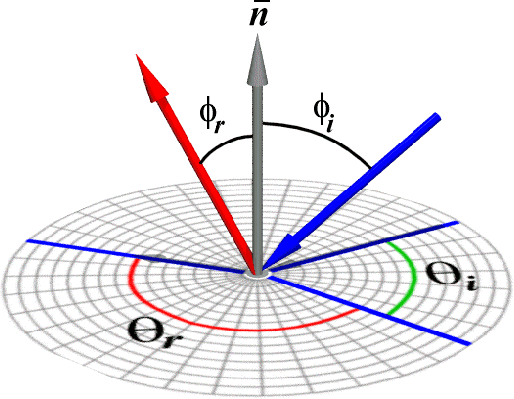
\includegraphics[width=9cm]{figures/brdf}
\caption[Esquema gráfico de la función bidireccional de distribución de reflectancia]{Esquema gráfico de la función bidireccional de distribución de reflectancia (BRDF). El par de ángulos de entrada ($\theta_{i},\phi_{i}$) define la dirección del rayo entrante, similarmente ($\theta_{r},\phi_{r}$) representan la dirección del rayo saliente. La función calcula la cantidad de radiancia emitida en la dirección del rayo saliente, a partir de la dirección del rayo entrante.}
\label{fg:brdf}
\end{figure}

Diversos fenómenos tienen lugar cuando un rayo de luz impacta una superficie de un objeto. En su máxima expresión, una BRDF podría tomar en consideración variables como la longitud de onda, la posición de salida del rayo reflejado en la superficie (modelando de esta forma dispersión interna en el material), e incluso el tiempo de demora entre la entrada y la salida del rayo.
De esta forma sería posible modelar fenómenos tan complejos como la fosforescencia y la polarización.

Una complejidad tal no resulta práctica en computación gráfica, por lo cual deben realizarse simplificaciones sobre los materiales subyacentes.
Una simplificación muy común de esta función consiste en ignorar los fenómenos anteriores y limitar la definición de la BRDF a un par de ángulos de entrada y de salida, para cada punto de la superficie, como se muestra en la Fig. \ref{fg:brdf}.
De cualquier manera, esta simplificación es todavía una función de {\em seis} variables, que incluye las cuatro dimensiones definidas por las direcciones de entrada y de salida, y las dos que se corresponden a una representación paramétrica de una superficie.

Debido a la prohibitiva complejidad aún presente en estas simplificaciones, los primeros modelos utilizados en computación gráfica eran funciones analíticas \cite{Phong1975,Blinn1977}, es decir, una función simple que no requería almacenamiento de datos (ya que el valor se calcula en el momento de llamar a la función).
De esta manera fue posible representar diversos materiales sencillos, sobre todo metales y objetos con una marcada reflectancia.
Las funciones no estaban basadas en ningún procedimiento de obtención, sino más bien en un procedimiento artístico que producía resultados aceptables.

Posteriormente surgieron modelos más precisos, los cuales desarrollaron funciones analíticas teniendo en consideración mayores precisiones sobre los modelos geométricos subyacentes, por lo que resultaron más ajustadas a los fenómenos reales \cite{He1991,Ward1992,Lafortune1997}.
Para esto, se modelaron las anisotropías en la reflectancia presentes en las superficies (reflectancia diferente para distintos ángulos).
En otras palabras, la inclusión de no linealidad otorga un mayor realismo.

Otros trabajos \cite{Dana1999,Matusik2003} realizaron mediciones de la reflectancia de materiales por medio de dispositivos de captura (goniorreflectómetros), lo cual constituye una solución de fuerza bruta, pero adecuada en algunos casos.
Los datos de las mediciones del material generalmente son publicados para uso de la comunidad gráfica y científica.

Finalmente, se ha intentado representar los datos mesurados en materiales reales con modelos matemáticos, buscando reducir costos de almacenamiento \cite{Ngan2005}.
En estos casos, por medio de modelos estándar de BRDFs, o por una combinación de los mismos, se buscan explicar los datos obtenidos en las medidas, con lo cual no es necesario almacenar la información capturada, sino que la misma se calcula a partir de la definición del nuevo modelo.
Si bien no es posible explicar {\em la totalidad} de los datos obtenidos, generalmente se obtienen buenas aproximaciones por medio de estos métodos, las cuales explican gran parte de los datos observados.

\subsection{Definición}
Previamente definimos la BRDF como una función matemática que tomaba como parámetro tres puntos del espacio.
Una forma equivalente consiste en definir, para cada punto de una superficie, el ángulo de entrada y salida del rayo

$$\rho(\theta_{i},\phi_{i},\theta_{r},\phi_{r}) = \frac{dL_{r}(\theta_{r},\phi_{r})}{dE_{i}(\theta_{i},\phi_{i})},$$

donde $E_{i}$ es la {\em irradiancia} entrante, que se define como flujo incidente sobre unidad de área, y $L_{r}$ es la radiancia reflejada.
Intuitivamente, la BRDF mide la cantidad de luz reflejada a partir de la cantidad de energía incidente en la superficie, para cada ángulo de entrada y de salida.

Muchas BRDF modelan por separado determinadas características comunes en materiales.
Por ejemplo, las contribuciones especulares (reflejos perfectos) y difusa (la luz se disipa en todas las direcciones de manera equitativa).
La primera produce diferencias visibles en superficies, siendo característica la visualización de círculos o líneas blancas sobre determinadas direcciones en las que se posiciona el observador.

La Fig.~\ref{fg:contribuciones} muestra ejemplos de estos rebotes.
Las direcciones de reflejo suelen formar patrones llamados lóbulos, los cuales permiten entender intuitivamente el comportamiento de la BRDF (a simple vista, es posible saber la dirección donde se dirigirán más rayos y por lo tanto, mayor radiancia).
Si el observador se coloca en la dirección de reflejo de estos lóbulos, observará mayor radiancia que en otras direcciones.

\begin{figure}
\center
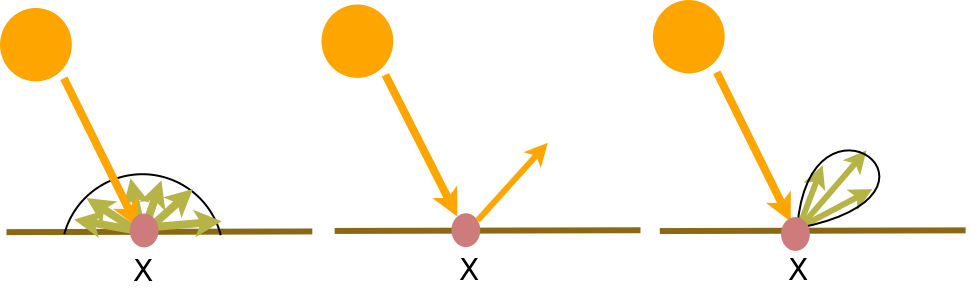
\includegraphics[width=11cm]{figures/contribuciones}
\caption[Diferentes reflectancias en BRDFs]{Diferentes reflectancias en BRDFs. La imagen de la izquierda muestra una reflexión difusa, la del centro, una completamente especular, y la de la derecha, lobular.}
\label{fg:contribuciones}
\end{figure}

La Fig.~\ref{fg:microestructura} muestra un ejemplo de una geometría microscópica de un material y su BRDF resultante.
Como puede observarse, la apariencia final de la BRDF depende de la orientación de determinadas estructuras presentes a escalas microscópicas del material.
En algunos casos es posible asumir distribuciones estadísticas, pero en la mayoria de los materiales esto no es así.
La microgeometría es lo suficientemente compleja como para presentar anisotropías y formas de apariencia caprichosa.
Como fue dicho, si no es posible modelar matemáticamente el comportamiento del material, muchas veces se recurre a mediciones sobre muestras reales.


\begin{figure}
\center
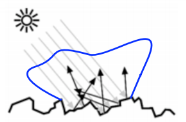
\includegraphics[width=5cm]{figures/microestructura}
\caption{Explicación del comportamiento observable en BRDFs.}
\label{fg:microestructura}
\end{figure}


\subsection{BRDF de Phong}
Un ejemplo muy común de BRDF analítica es el modelo de Phong, ver Fig~\ref{fg:phongVecs}, el cual presenta la siguiente definición matemática:

$$\rho_{phong}(-L,V) =  k_{a} I_{a} + k_{d} max((N \cdot L),0) + k_{s} (R \cdot V)^{\alpha},$$

donde $k_{a}$, $k_{d}$ y $k_{s}$ son coeficientes de iluminación ambiente, difusa y especular, el vector $N$ es el normal a la superficie, $R$, el reflejado (en un rebote especular), $V$ el vector  que se forma desde la superficie hacia la posición del observador y $L$ el vector desde la superficie hacia la fuente de luz (por lo que debe tomarse su opuesto, $-L$, para hacer la definición compatible con la definición de BRDF), y $\alpha$ es un parámetro que determina el brillo final de los reflejos del material (llamado {\em glossiness}), ver Fig.~\ref{fg:phongparametros}.


\begin{figure}
\center
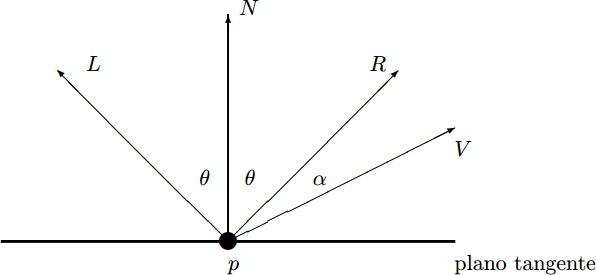
\includegraphics[width=11cm]{figures/phongVecs}
\caption[Vectores intervinientes en el cómputo de la BRDF de Phong]{Vectores intervinientes en el cómputo de la BRDF de Phong. La radiancia ingresa desde $-L$ hacia $p$. El observador se encuentra en $V$.}
\label{fg:phongVecs}
\end{figure}

El término ambiente en la ecuación, representa una aproximación a la radiancia dispersa por toda la escena, y está definido por una constante.

El término difuso de la BRDF del material no cambia respecto de la posición del observador.
La misma es resultado de la normal a la superficie y la posición de la fuente de luz.
En un extremo, el término difuso se hace cero cuando la luz incide perpendicularmente a la superficie.
El otro extremo se da cuando la normal coincide con la fuente de luz, en cuyo caso el término difuso es máximo.

El único cambio que puede percibir un observador al moverse, en la apariencia de una superficie que utiliza la BRDF de Phong, está dado en el término especular.
Intuitivamente, a medida que el observador en $V$ se posiciona más cerca de la dirección del rayo reflejado $R$, ocurre que $R$ es más parecido a $V$, llegando en el límite a $R = V$
y por lo tanto $R \cdot V$ es máximo.
A medida que el observador en $V$ se aleja de $R$, el producto escalar tiende a cero, y la reflectancia se percibe en menor medida.

Si bien el modelo es mayormente fenomenológico, el mismo es flexible e intuitivo.
Además, obtiene buenos resultados en superficies opacas de marcada especularidad, como metales y plásticos, entre otros.

\begin{figure}
\center
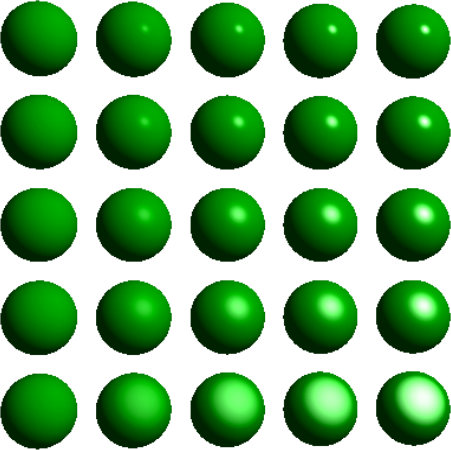
\includegraphics[width=9cm]{figures/phongparametros}
\caption[Diferentes apariencias en el modelo de Phong]{Diferentes apariencias obtenidas en una esfera, cambiando parámetros en el modelo de Phong, para un observador y una fuente de luz fijos. De izquierda a derecha $k_{s}$ varía de $0$ a $1$. De arriba hacia abajo, $\alpha$ varía de $50$ a $1$.}
\label{fg:phongparametros}
\end{figure}

%\subsection{Radiosidad}

%\subsection{Ray Tracing}
%\subsection{Ray Marching}
%\subsection{Volume Rendering}
%\subsection{Photon Mapping}

\section{Materiales específicos}
Debido a la necesidad creciente en el modelado y renderizado realista de materiales, el diseño de BRDFs y métodos derivados de las ecuaciones del renderizado, y del renderizado de volúmenes, evolucionaron hacia representaciones más complejas, permitiendo representar una mayor cantidad de apariencias y materiales.
Además, y debido a las características particulares de determinados materiales, los métodos mencionados resultaron inadecuados de ser aplicados de manera directa.
Esto provocó que se desarrollaran técnicas específicas para materiales determinados.

En otras palabras, si bien las ecuaciones presentadas proveen un marco teórico general de los fenómenos que ocurren entre la energía radiante y los materiales en una escena, los detalles de implementación computacional (representación como superficie o volumen, escala de representación, consideraciones de almacenamiento, etc.) muchas veces hacen imposible una utilización directa de las mismas, debiendo diseñarse soluciones particulares que atiendan a los requerimientos específicos de cada material.
Por ejemplo, la BRDF no siempre resulta ser la solución adecuada para modelar todas las superficies, prefiriéndose una BSSRDF o una BTF en algunos casos.

Debido a esto han surgido técnicas que han considerado distintos aspectos a la hora de obtener un renderizado realista.
Algunas han optado por sintetizar modelos de primeros principios. 
Entre ellas se encuentran modelar el proceso de fabricación del material (por ejemplo en telas), o modelizar el comportamiento químico de determinados componentes que forman el material (piel).
Otras metodologías utilizaron un enfoque fenomenológico para la obtención de un modelo.
Entre estas técnicas encontramos el diseño de las microgeometrías presentes en superficies de materiales (cerámicos), y el uso de dispositivos de captura de determinadas propiedades del material (pinturas de autos). 


Esta sección presenta distintos ejemplos de diseño de materiales en computación gráfica con diversas metodologías.
Se desprende que el modelado y renderizado de materiales es aún un tema abierto, del cual sólo algunos ejemplos han sido desarrollados \cite{Dorsey2007}.
Existe aún un amplio abanico de materiales que requieren tratamiento.
Dependiendo del nivel de realismo deseado, es posible aplicar diversas metodologías al diseño de los mismos.


\subsection{Piel}
Comenzaremos con un material extremadamente complejo y ubicuo en computación gráfica: la piel humana.
Debido a su extenso uso en aplicaciones gráficas, existen para este material un importante número de trabajos científicos, los cuales varían en complejidad, presentando diversos enfoques a la hora de realizar su modelado.
Un modelo poco preciso de la piel puede ser fácilmente detectado por humanos, por lo cual un diseño cuidado es necesario para alcanzar un realismo aceptable.


La composición de la piel está fuertemente estudiada en medicina.
Debido a esto, existen trabajos muy completos sobre su estructura y propiedades \cite{Walters2002}.
La piel está compuesta por diversas capas como la epidermis, la dermis y la hipodermis.
La más exterior es la epidermis, compuesta por células muertas.
La siguiente capa en profundidad es la dermis, la cual es más ancha y posee vasos sanguíneos (lo cual afecta, entre otras consideraciones, el color final de la piel).
La hipodermis es la capa más interna y conecta la piel con el cuerpo.
Todas estas capas presentan una estructura muy compleja.
Este material es muy dinámico, y puede ser afectado por diversos factores, como el sol, lastimaduras, y cambios en el torrente sanguíneo.
Su estructura geométrica también es compleja, presentando poros y por ejemplo, patrones característicos que varían para cada persona (por ejemplo las huellas dactilares).

La estructura de capas fue imitada en computación gráfica realizando abruptas simplificaciones.
De esta forma, se diseñó un modelo de reflectancia para su superficie (BRDF) y un modelo de dispersión debajo de la superficie (\acrshort{BSSRDF}) en una segunda capa, junto con un modelo microgeométrico de la superficie.

Un ejemplo es \cite{Marschner2000}, el cual utiliza una BRDF de Lafortune (la cual es una generalización de la BRDF de Phong con varios lóbulos) para la reflectancia superficial, junto con texturas que se mapean sobre una geometría de la cara de una persona.
En otro trabajo se utilizó además información proveniente de moldes de polímeros presionados sobre la cara de personas \cite{Haro2001}, con el fin de capturar detalles finos de la geometría, utilizando además algoritmos de síntesis de imágenes para generar muestras más grandes que las medidas, ver Fig.~\ref{fg:piel}.

\begin{figure}
\center
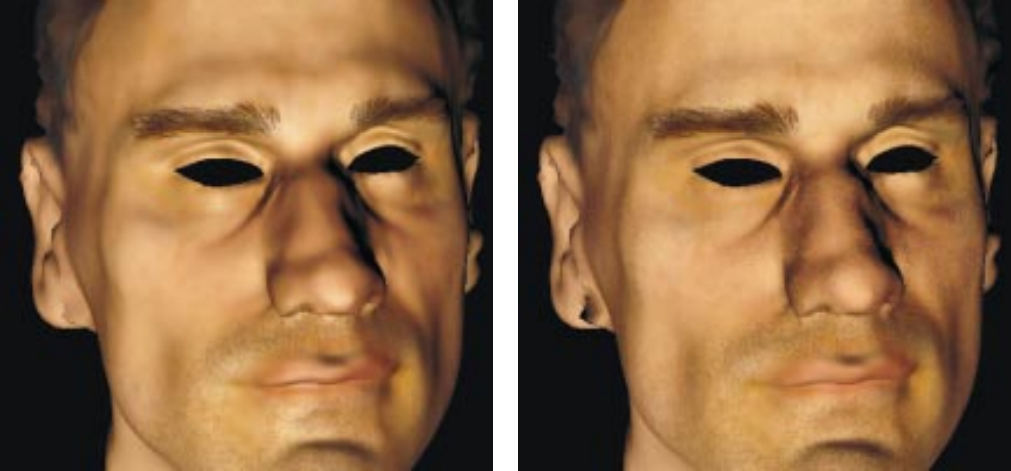
\includegraphics[width=9cm]{figures/piel}
\caption[Piel Humana renderizada]{Piel Humana renderizada con el método de \cite{Marschner2000}. La imagen de la derecha muestra la mejora obtenida al agregar detalles de geometría fina en el modelo (nariz, parte inferior del labio).}
\label{fg:piel}
\end{figure}

Un modelo basado en primeros principios puede verse en \cite{Krishnaswamy2004}.
En dicho trabajo se definen geometrías precisas para la dermis y epidermis, a partir de la cual se realizan simulaciones físicas estocásticas de rebote de la luz (simulaciones Monte Carlo), gracias a las cuales es posible reconstruir una BRDF.
El modelo incluye muchos otros detalles de los procesos físicos intervinientes, como la intervención de la melanina y la bilirrubina, además de consideraciones de absorción, pigmentación, etc.

Existen trabajos que abordan otros aspectos del modelado de la apariencia de la piel.
El estudio de los patrones que produce el envejecimiento es sujeto de estudio en \cite{Boissieux2000}.
Los mismos fueron medidos en muestras reales de una empresa cosmética.
También es posible obtener información geométrica fina a partir de imágenes \cite{Golovinskiy2006}.

Este ejemplo muestra con claridad que un mismo material puede presentar una amplia gama de modelos que simulan su apariencia, dependiendo de la aplicación específica y los detalles que se buscan representar.

\subsection{Materiales Porosos}

Determinados materiales porosos presentan micro-poros en la geometría de sus superficies.
Estos poros afectan de manera directa la noción de superficie contínua, asumida al modelar un material como una superficie y representar su comportamiento con la energía radiante por medio de una BRDF.

Estos poros microscópicos son aún más pequeños que los poros presentes en la piel humana.
Si bien su tamaño es mayor que la longitud de onda de la luz, los mismos no son visibles al ojo humano.

Entre los pocos trabajos sobre estos materiales, se encuentra el de Merillou \cite{Merillou2000}.
En dicho trabajo la definición estándar de BRDF es modificada para incluir términos matemáticos que representan la estructura y el comportamiento de materiales porosos.
Para esto se modifican los coeficientes especular ($k_{s}$) y difuso ($k_{d}$) de la BRDF, transformándolos en una {\em función} dependiente del ángulo de entrada y la posición del observador.

La idea intuitiva detrás de estas modificaciones es profundizar el modelo sobre dichos coeficientes, teniendo en cuenta el efecto de los poros sobre los mismos, debido a que la existencia de éstos puede modificar el comportamiento de los rayos de luz.
Por ejemplo, un rayo de luz que se comporta de forma especular, podría ser desviado por un poro y resultar en energía difusa.
Esto se traduce en la dirección del rayo de rebote, ya que la presencia del poro provoca que el rayo que sería especular obtenga una dirección de salida posiblemente arbitraria.
Matemáticamente, el coeficiente difuso toma una parte del coeficiente especular.

Para obtener una distribución estadística de las geometrías de los poros presentes en una superficie, se deben modelizar los mismos.
El modelado de los poros se lleva a cabo por medio de simulaciones estocásticas Monte Carlo sobre posibles geometrías microscópicas de poros bajo ciertas asunciones.
Dos ejemplos diferentes de poros pueden observarse en la Fig.~\ref{fg:poro}.
Se simula el rebote de rayos de luz sobre la geometría sintetizada, computándose las distribuciones de reflectancia para poros con distintas formas, utilizando un máximo en el número de rebotes.
También es posible tener en cuenta un factor de absorción en cada rebote, lo cual disminuye la radiancia del rayo siendo computado.
El proceso se repite para distintas simulaciones estocásticas de la geometría de los poros.


En la Fig.~\ref{fg:ceramico} podemos observar una imagen de una maceta renderizada con una BRDF tradicional, y a la derecha, la misma imagen utilizando la BRDF modificada por este método.

\begin{figure}
\center
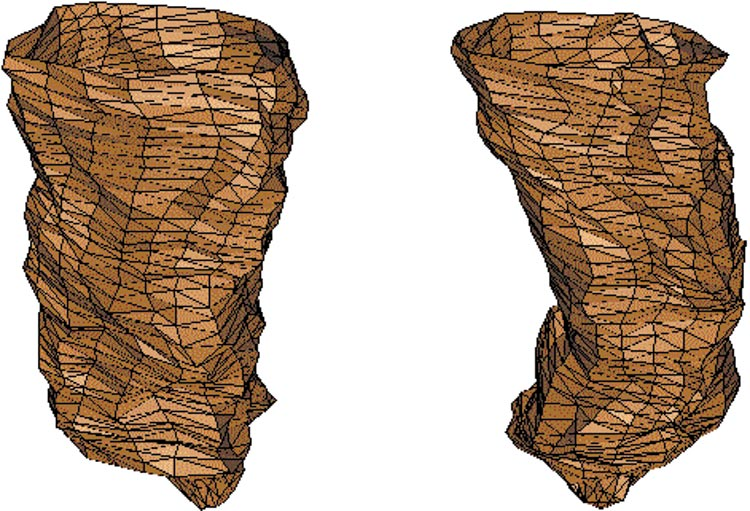
\includegraphics[width=8cm]{figures/poro}
\caption[Poros sinterizados]{Ejemplo de poros sintetizados utilizando el método desarrollado en \cite{Merillou2000}.}
\label{fg:poro}
\end{figure}

\begin{figure}
\center
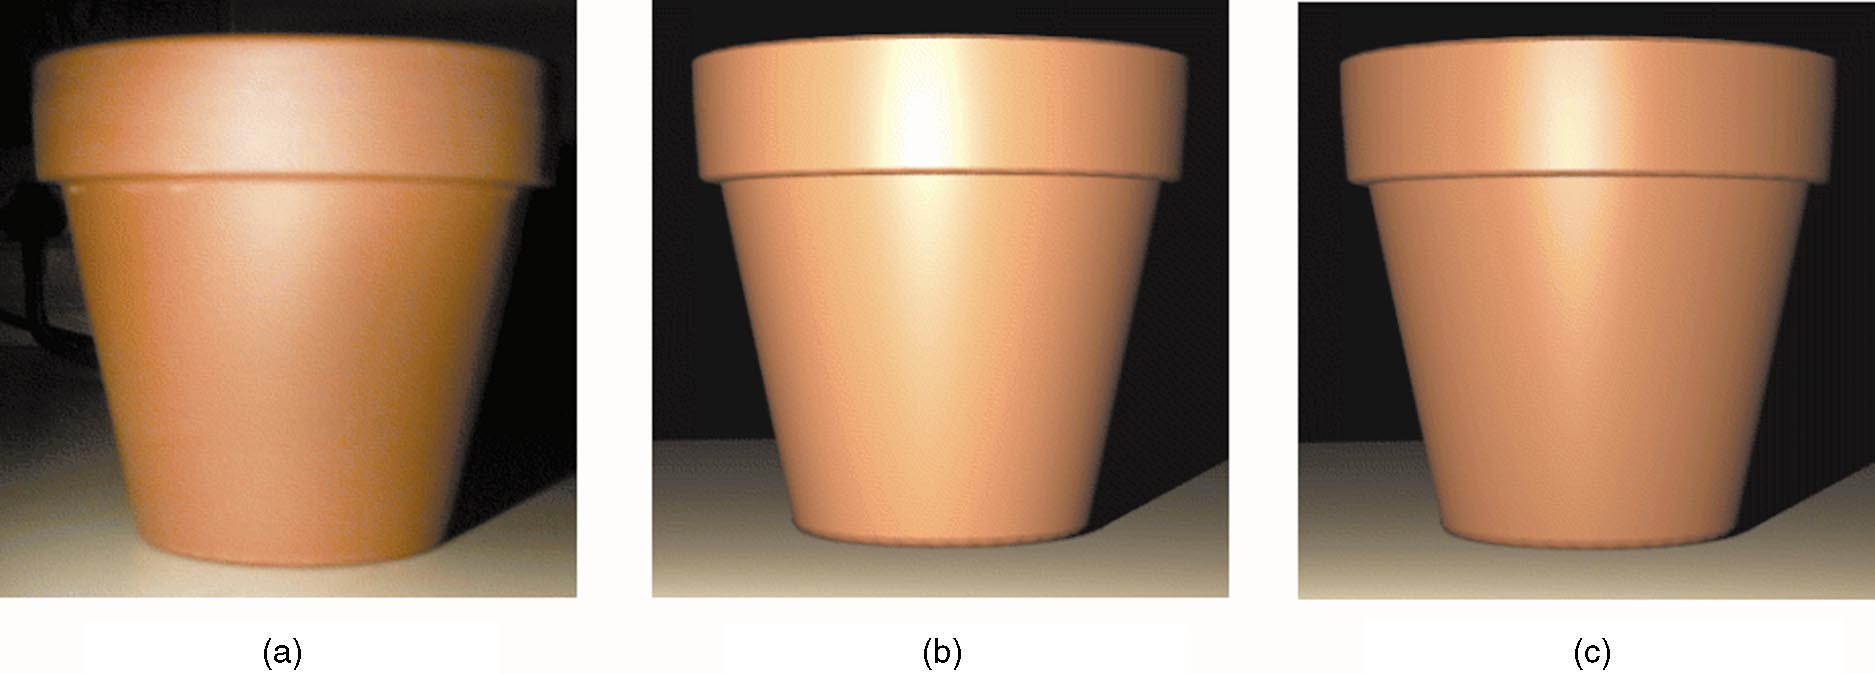
\includegraphics[width=11cm]{figures/ceramico}
\caption[Cerámicos renderizados]{Cerámicos renderizados. Izquierda: maceta real. Centro: utilizando una BRDF tradicional. Derecha: utilizando el método propuesto en \cite{Merillou2000}.}
\label{fg:ceramico}
\end{figure}

La tesis presente se ubica sobre este tipo de materiales, dado que el pan es un material poroso que involucra cocción previa.
A diferencia de los cerámicos, los poros son visibles por el ojo humano.

\subsection{Pelo}
Al igual que con los cerámicos y la piel, el modelado del pelo debe tener en cuenta su estructura interna.
Cada pelo individual consiste de tres partes principales: una médula central, el córtex y una cutícula exterior.
Su color está dado por gránulos de melanina en el córtex.
Cuando no están presentes estos gránulos se observa un color blanco.


Existen dos tipos principales de pelo, uno es el vello, el cual crece en prácticamente todo el cuerpo, con $1$ {\em mm} de alto, y otro es el pelo terminal, el cual se encuentra en el cuero cabelludo.
Este último fue el que recibió mayor atención en computación gráfica.
El pelo terminal tiene aproximadamente entre $50$ y $90$ micrones de diámetro.
Existen entre $175$ y $300$ pelos terminales por {\em $cm^{2}$}.
El pelo de animales difiere del humano en color, tamaño, y densidad.

Cada pelo individual puede considerarse una superficie con dispersión lumínica propia.
Por otro lado, la apariencia típica del pelo está dada por el conjunto de muchos pelos individuales.
Sin embargo, utilizar soluciones volumétricas típicas, como modelar el pelo como se modela una nube o el humo no resulta adecuado, ya que la geometría del pelo afecta la reflectancia de la luz incidente.

Para solucionar estos inconvenientes se creó una estructura denominada {\em texel}, que no debe confundirse con un elemento de una textura.
Un texel es una {\em estructura de datos} volumétrica que asocia tres componentes: una densidad de área proyectada $\rho$, un marco de referencia $\bold{B}$ y un modelo bidireccional de reflexión de la luz $\psi$, a cada posición $3D$ del espacio.
La densidad de área proyectada $\rho$ es la fracción del área proyectada del {\em vóxel} (cada entrada en una matriz tridimensional) en una dirección particular que es cubierta por geometría del pelo proyectada en la misma dirección.
En $\bold{B}$, la orientación queda especificada por los vectores normal, binormal, y tangente.
Para determinar los vectores, se asume un cilindro general que crece desde la piel del cuero cabelludo.
$\psi$ se define como una variación del modelo de Phong, devolviendo la luz reflejada en el punto.
Los componentes difuso y especular del modelo son,

\begin{align*}
\psi_{d} &= K_{d} sin \theta_{i}\\
\psi_{s} &= K_{s} (cos \theta_{i} cos \theta_{r} + sin \theta_{i} sin \theta_{r})^{p},
\end{align*}

donde $\theta_{i}$ es el ángulo entre la luz y la tangente al pelo, y $\theta_{r}$ es el ángulo entre la tangente al pelo y el observador.

Luego, para calcular el color final de un pixel en pantalla, desde el punto de vista del observador, se recorren en línea recta, desde $t_{near}$ a $t_{far}$ según corresponda a ese pixel, los texels necesarios,

$$L = \sum_{t=t_{near}}^{t=t_{far}} {e^{-\tau \sum_{u=t_{near}}^{u=t} \rho(u)} \rho(t) \sum_{i} L_{i}(t) \bold{\psi}(t)},$$

donde la suma sobre $i$ refiere a las fuentes de luz, y $\tau$ es un coeficiente que convierte las distribuciones de área proyectada en un coeficiente de atenuación.

Este método sirve para simular pelo corto, pero visto a cierta distancia, ver Fig.~\ref{fg:osopelo}.
La percepción de pelo se pierde cuando la cámara se acerca demasiado al objeto.

\begin{figure}
\center
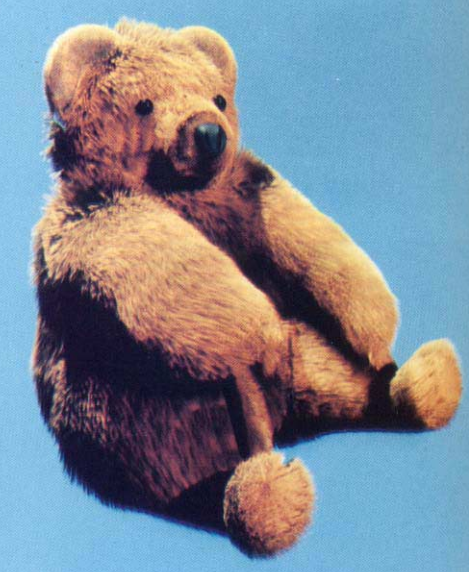
\includegraphics[width=6cm]{figures/osopelo}
\caption[Renderizado de pelo en un oso de peluche]{Ejemplo de renderizado de pelo en un oso de peluche con el método propuesto en \cite{Kajiya1989}.}
\label{fg:osopelo}
\end{figure}

%The projected area density is the fraction of the projected area of the voxel in a particular direction that is covered by hair geoemetry projected in the same direction

Es posible mejorar el método por medio de otras funciones $\bold{\psi}$, teniendo en cuenta factores como la transmitancia y el impacto de las fibras individuales entre sí (iluminación indirecta).
Puede verse un estudio más completo de la literatura sobre renderizado de pelo en \cite{Ward2007}.

\subsection{Telas}
Las telas son un material similar al pelo en cuanto a su composición, ya que están formadas por un conjunto de fibras.
Las fibras de telas presentan diferentes {\em tinturas}.
Es importante considerar las tinturas que componen una fibra para entender la apariencia de una tela cuando es vista desde distintos ángulos.
Por ejemplo, determinadas fibras de telas presentan más de una tintura, como muestra la Fig.~\ref{fg:fibra}.
En este caso, los rayos de luz que llegan desde distintas posiciones atraviesan distintas longitudes sobre las tinturas, produciendo iridiscencia, es decir, cambio de color visible dependiendo del ángulo de visión.

\begin{figure}
\center

\includegraphics[width=4cm]{figures/fibra}
\caption[Ejemplo de fibra de tela con más de una tintura]{Ejemplo de fibra de tela con más de una tintura. Se puede observar una tintura roja en el centro, y una tintura azul que la envuelve.}
\label{fg:fibra}
\end{figure}

La apariencia de cada tipo de tela es diferente, y depende del material utilizado (seda, lana, hilos, etc.) como del proceso de tejido en sí.
En \cite{Xu2001} se observa que determinados hilos están formados por un conjunto de fibras compactadas y con estructura helicoidal.
Esta observación es utilizada para definir un texel específico como en el caso del pelo, el cual luego permite determinar la cantidad de luz que será emitida en una dirección para una dirección entrante, ver Fig. \ref{fg:tela}.
Para esto se tienen en cuenta efectos como sombras, oclusión y dispersión múltiple entre los distintos hilos que componen una tela.
Debe contarse además con una estructura coherente que conecte a los hilos, formando una tela realista.
Para esto se utilizan curvas $3D$ construídas a partir de los puntos de control definidos en la división de la superficie.


\begin{figure}
\center
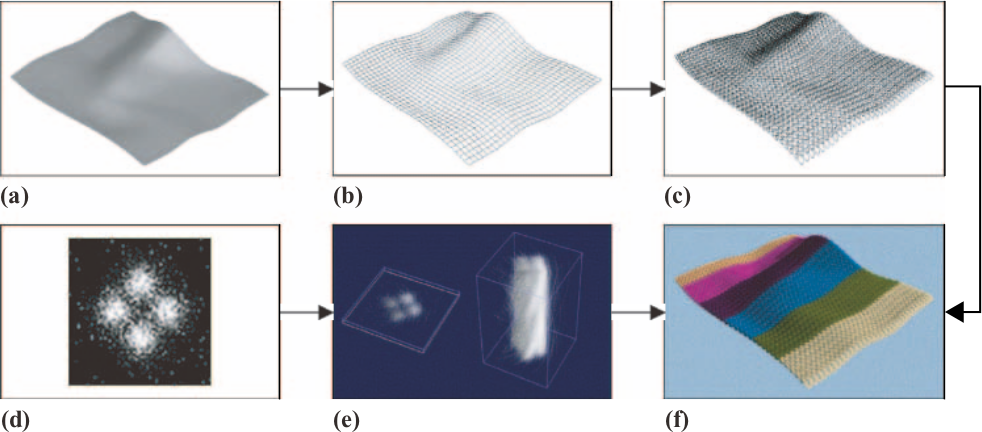
\includegraphics[width=13cm]{figures/tela}
\caption[Pasos para la definición de un modelo de una tela]{Pasos para la definición de un modelo de una tela, donde se toman en cuenta fibras individuales. Además de la utilización de una superficie (a), la misma se subdivide (b) para alojar distintas estructuras de hilo (c), los cuales se modelan individualmente ((d) y (e)).}
\label{fg:tela}
\end{figure}

\subsection{Pinturas de autos}
Determinadas marcas de automotores han expuesto la necesidad de una correcta visualización de las pinturas aplicadas sobre la superficie exterior de los mismos.
Los modelos desarrollados se han utlizado para presentar al público nuevos productos de estas fábricas, permitiendo a los posibles compradores configurar los colores y características deseadas en las pinturas.
Debido a esto, es deseable un buen modelo del material en computación gráfica, que permita luego una reproducción lo más fiel posible al mismo, en un automóvil real.

Se han desarrollado principalmente dos categorías de métodos para obtener un material con la apariencia de pintura de automóviles: aquellos basados en primeros principios \cite{Ershov2001}, y los basados en capturas de características de pinturas reales.

En el primero se realiza un modelo por capas, donde cada capa contiene partículas de pigmentos como en las pinturas reales.
El modelo de dos capas presentado asume una capa con partículas que reflejan la luz especularmente, y la otra con una pintura opaca.
Tomando en consideración parámetros como la densidad, la distribución de las orientaciones de las partículas, la transmitancia y la reflectancia, derivan una compleja BRDF parametrizada y analítica que permite definir distintos tipos de pinturas, ver Fig.~\ref{fg:pinturaauto}.

En el caso de datos mesurados, es posible utilizar distintas tomas de la radiancia saliente de la pintura de autos para combinarlas en un modelo.
En \cite{Dumont2001} además se utilizan texturas que representan la microgeometría de las pinturas También se utilizó ruido para producir efectos como el denominado {\em brillo} (sparkle).
En otro trabajo \cite{Gunther2005}, se utilizaron los datos de las medidas para producir un modelo analítico estadístico del brillo.
Como puede verse, es posible utilizar diversas metodologías para producir el mismo material o el mismo efecto.
La elección final se hace en base a la complejidad de la captura, costos computacionales, objetivos, y el realismo resultante, entre otros factores.

\begin{figure}
\center
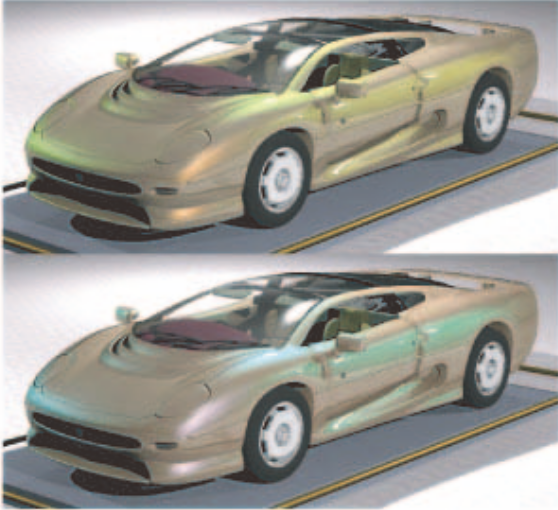
\includegraphics[width=8cm]{figures/pinturaauto}
\caption[Pinturas de autos diseñadas utilizando primeros principios]{Pinturas de autos diseñadas utilizando primeros principios en \cite{Ershov2001}. Cambiando un parámetro pueden obtenerse diferentes apariencias (en este caso, el ancho de las capas de interferencia).}
\label{fg:pinturaauto}
\end{figure}


\section{Conclusiones}
En este capítulo presentamos un resumen del estado del arte en modelado y renderizado de materiales en computación gráfica.
Del capítulo se desprende que para lograr un modelo realista de un material dado, es necesario modelizar tanto su geometría como su interacción con la luz, de la manera más realista posible.
Además, deben tenerse en cuenta los costos computacionales, la escala de la representación buscada, y el método utilizado para el renderizado del mismo (utilizar la ecuación del renderizado, modelando el material como una superficie, o diseñar el mismo como un volumen).

El pan ha sido un material elusivo en computación gráfica.
Se cuenta con un único trabajo en el tópico \cite{Tong2005}.
El enfoque utilizado es la fuerza bruta, es decir, capturas de reflectancia e imágenes de la miga de pan desde un punto de vista puramente fenomenológico.
Además, no se realizan consideraciones sobre la geometría del mismo.
Estas y otras limitaciones severas del método fueron superadas en la presente tesis.

En los capítulos que siguen, mostraremos como el diseño de la geometría y la interacción lumínica, fueron claves para lograr un renderizado realista de la miga y corteza de diferentes tipos de panes.

